%%% Folie
\begin{frame}{Leitfragen des heutigen Kapitels}
    \begin{block}{Den Raspberry Pi mit Strom versorgen}
        \begin{itemize}
            \footnotesize
            \setlength\itemsep{.5em}

            \item Wie viel Strom benötigt der Raspberry Pi?
            \item Wie lange hält die Batterie bzw. der Akku?
            \item Was kostet der jährliche Stromverbrauch?
        \end{itemize}
    \end{block}

    \begin{block}{Signale verarbeiten und erzeugen}
        \begin{itemize}
            \footnotesize
            \setlength\itemsep{.5em}

            \item Welche Arten der Signalübertragung gibt es?
            \item Welche Signalarten kann der Raspberry Pi verarbeiten?
            \item Wie werden Sensoren/Aktoren mit dem Raspberry Pi verbunden?
            \item Wie lassen sich Hardwareschäden dabei vermeiden?
            \item Wie lassen sich inkompatible Logikpegel anpassen?
        \end{itemize}
    \end{block}

    \begin{block}{Mechanische Arbeit verrichten}
        \begin{itemize}
            \footnotesize
            \setlength\itemsep{.5em}

            \item Wie viel Strom kann der Raspberry Pi bereitstellen?
            \item Wie können stärkere Lastströme geschaltet werden?
        \end{itemize}
    \end{block}
\end{frame}

%%% Folie
\begin{frame}{Lernziele}
    \begin{block}{Physikalische Grundlagen}
        \begin{itemize}
            \footnotesize
            \setlength\itemsep{.5em}

            \item Eine einfache Definition des elektrischen Stroms kennen und verstehen
            \item Die Begriffe ,,Spannung'', ,,Stromstärke'' und ,,Widerstand''' erklären
            \item Die Unterschiede zwischen ,,Gleichstrom'' und ,,Wechselstrom'' kennen
            \item Das Ohmsche Gesetz anwenden können
        \end{itemize}
    \end{block}

    \begin{block}{Stromversorgung für den Pi}
        \begin{itemize}
            \footnotesize
            \setlength\itemsep{.5em}

            \item Die Anforderungen des Raspberry Pi an die Stromversorgung kennen
            \item Die Funktionsweise eines typischen USB-Netzteils verstehen
            \item Die Lebensdauer einer Batterie/Akku abschätzen können
            \item Den Verbrauch und die erwarteten Stromkosten berechnen können
        \end{itemize}
    \end{block}

    \begin{block}{Sensoren und Aktoren}
        \begin{itemize}
            \footnotesize
            \setlength\itemsep{.5em}

            \item Die am Raspberry Pi nutzbaren Signalarten erklären können
            \item Die Hardwareschnittstellen des Raspberry Pi nutzen können
            \item Analoge und digitale Sensoren und Aktoren verbinden können
            \item Stromstärken und Spannungen an den Raspberry Pi anpassen
        \end{itemize}
    \end{block}
\end{frame}

%-------------------------------------------------------------------------------
\section{Physikalische Grundlagen}
%-------------------------------------------------------------------------------

%%% Folie
\begin{frame}[allowframebreaks]{Was ist elektrischer Strom?}
    \begin{columns}
        \footnotesize

        \column{.6\textwidth}
        \raisebox{-0.5\height}{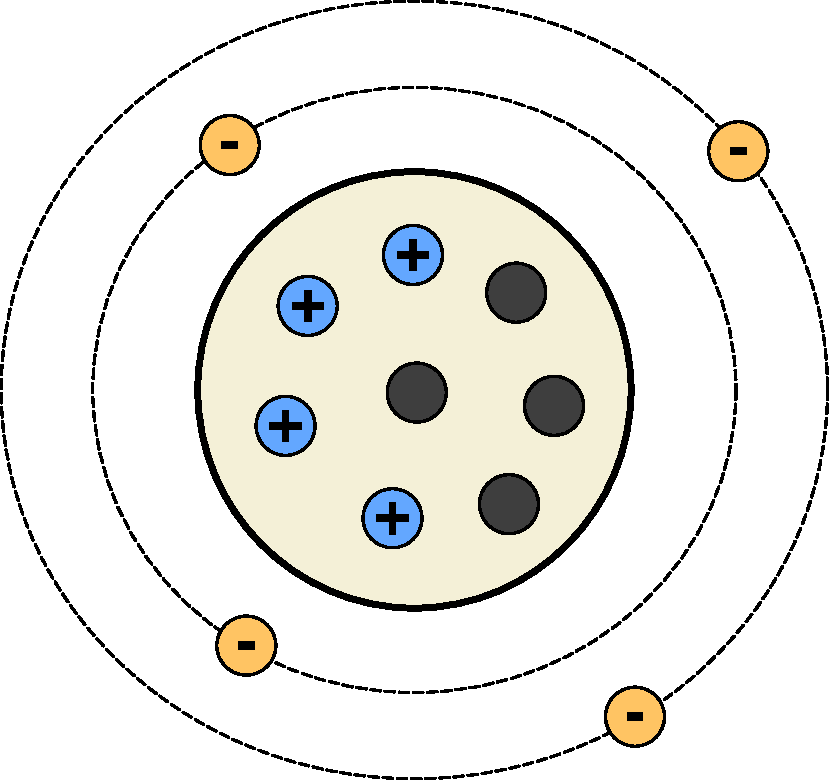
\includegraphics[width=.6\textwidth]{2-hardwaredesign/img/atom_detail}}

        \column{.4\textwidth}
        \raisebox{-0.25\height}{
\includegraphics[width=.4cm]{2-hardwaredesign/img/atom_kern}}
        \hskip 1em
        Atomkern \\
        \smallskip

        \raisebox{-0.25\height}{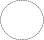
\includegraphics[width=.4cm]{2-hardwaredesign/img/atom_schale}}
        \hskip 1em
        Schale \\
        \bigskip

        \raisebox{-0.25\height}{
\includegraphics[width=.4cm]{2-hardwaredesign/img/atom_elektron}}
        \hskip 1em
        Elektron \\
        \smallskip

        \raisebox{-0.25\height}{
\includegraphics[width=.4cm]{2-hardwaredesign/img/atom_proton}}
        \hskip 1em
        Proton \\
        \smallskip

        \raisebox{-0.25\height}{
\includegraphics[width=.4cm]{2-hardwaredesign/img/atom_neutron}}
        \hskip 1em
        Neutron \\
    \end{columns}

    \bigskip
    \bigskip

    \parbox{\linewidth}{
        \scriptsize
        Am einfachsten lässt sich die Wirkungsweise des elektrischen Stroms verstehen,
        wenn man das alte, Bohrsche Atommodell betrachtet, bei dem jedes Atom in Analogie
        an unser Sonnensystem als ein Kern mit Protonen und Neutronen sowie diesen auf
        festen Bahnen umkreisenden Elektronen beschrieben wird.
        \smallskip

        Damit Strom in einem Material fließen kann, muss ein Teil der darin enthaltenen
        Elektronen mit geringem Energieaufwand frei beweglich sein. Man spricht dann von
        einem \textbf{Leiter}. Beispielsweise besitzen alle Metalle ein freies Elektron
        auf der äußersten Hülle, das leicht vom Atomkern gelöst werden kann.
        \smallskip

        In nicht-leitenden Materialien -- sog. \textbf{Isolatoren} -- gibt es keine frei
        beweglichen Elektronen, so dass ein großer Kraftaufwand zum Herauslösen benötigt
        wird. In \textbf{Halbleitern} kann die Anzahl der freien Elektronen während der
        Herstellung oder später durch äußere Umstände beeinflusst werden.
    }

    %%% Folie
    \framebreak

    \begin{columns}
        \column{\dimexpr\paperwidth-28pt}
        \begin{center}
            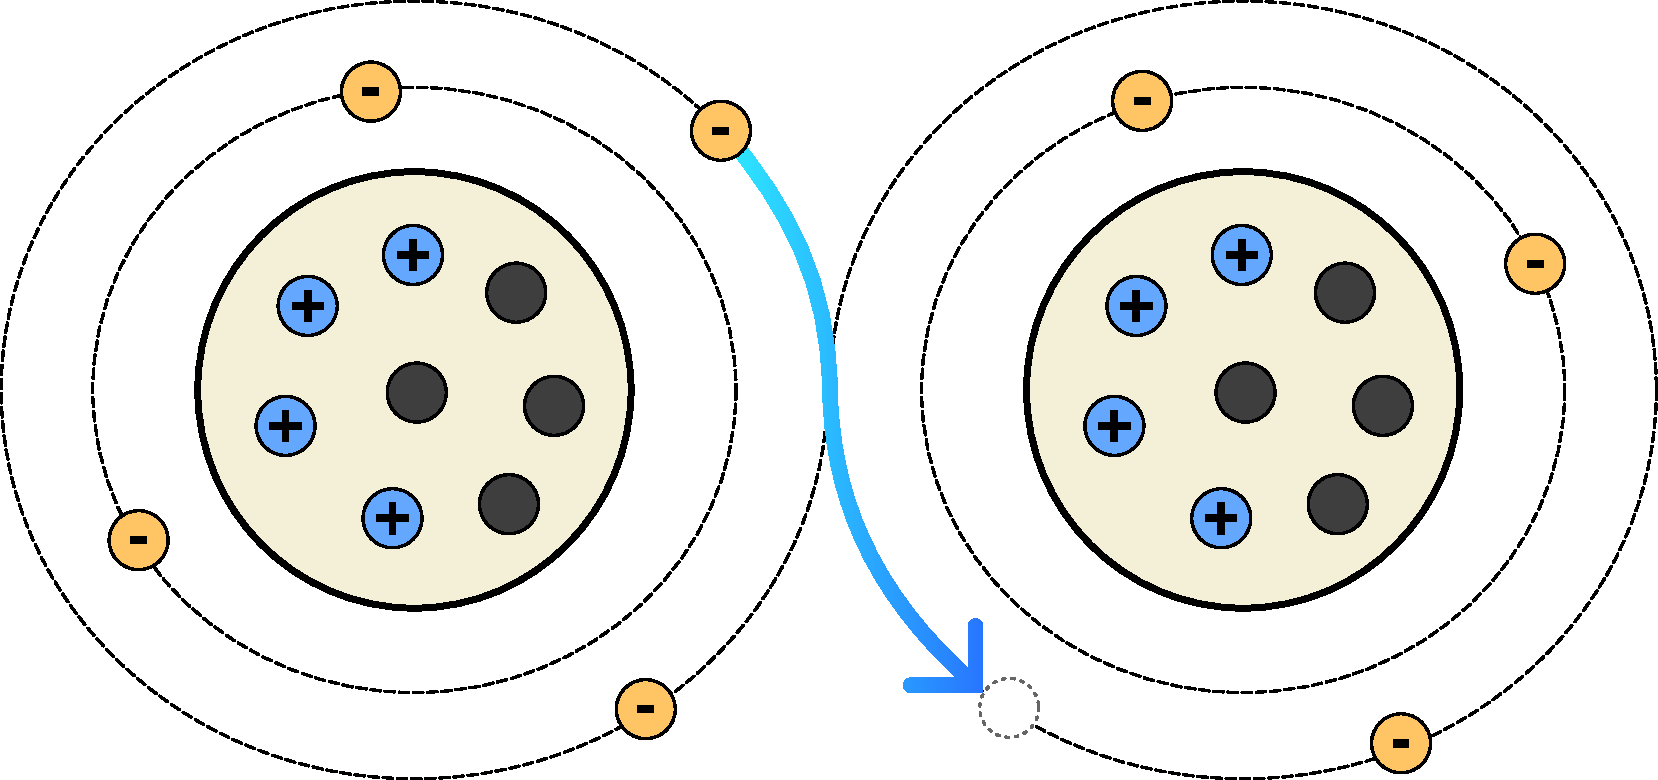
\includegraphics[width=.7\textwidth]{2-hardwaredesign/img/atom_elektronenfluss}
        \end{center}
    \end{columns}

    \bigskip

    \parbox{\linewidth}{
        \scriptsize
        Im Normalzustand sind die meisten Atome elektrisch neutral, da sie die
        gleiche Anzahl Protonen wie Elektronen besitzen. Atome mit einem Überschuss
        oder Mangel an Elektronen werden \textbf{Ionen} genannt und sind
        \textbf{elektrisch geladen}. Wurde beispielsweise ein Elektron aus der
        äußeren Hülle eines Atoms heraus gelöst, kann ein benachbartes Elektron
        überspringen, wodurch Strom fließt.
        \smallskip

        \textbf{Elektrischer Strom} entspricht somit der \textbf{Bewegung freier
        Elektronen} innerhalb eines leitfähigen Materials. Strom entsteht daher,
        indem die freien Elektronen durch \textbf{magnetische} oder
        \textbf{chemische Einwirkung} in Bewegung versetzt werden.
        Allerdings darf man das nicht nicht so vorstellen, dass ein Elektron
        geradlinig durch das Material hindurch wandert. Vier mehr nimmt es einen
        zufälligen Weg und schiebt dabei alle anderen Elektronen aus dem Weg,
        da sich Elementarteilchen mit gleicher Ladung immer abstoßen.
    }

    %%% Folie
    \framebreak

    \parbox{\linewidth}{
        \footnotesize
        Folgende Begriffe sind zur Beschreibung elektrischer Ströme von besonderer Bedeutung:
    }

    \begin{block}{Spannung \hfill (Voltage)}
        \smallskip
        \parbox{\linewidth}{
            \scriptsize

            Die Spannung wird immer \textbf{zwischen zwei Punkten} gemessen und beschreibt
            wie viele Elektronen auf der einen Seite zu viel oder auf der anderen Seite zu
            wenig sind. Sie beschreibt somit die \textbf{Ladungsdifferenz} zwischen den beiden
            Punkten und wird in der Einheit \textbf{Volt} gemessen. Sie liefert die Kraft,
            die auf die Elektronen ausgeübt wird, um sie in Bewegung zu setzen und ist
            (sofern die beiden Punkte über ein elektrisch leitendes Material verbunden sind)
            die \textbf{Ursache für den Stromfluss}.
        }
    \end{block}

    \begin{block}{Masse \hfill (Ground)}
        \smallskip
        \parbox{\linewidth}{
            \scriptsize

            Beschreibt in einem Stromkreis den gemeinsamen Bezugspunkt, vom dem aus alle andere
            Spannungen gemessen werden. Entspricht bei einer Batterie meistens dem Minuspol oder
            beim Hausstrom dem Neutralleiter. In einem Stromkreis fließt der Strom gedanklich
            immer vom Pluspol der Stromquelle zur Masse, die meist dem Minuspol der Stromquelle
            entspricht.
        }
    \end{block}

    \begin{block}{Stromstärke \hfill (Current)}
        \smallskip
        \parbox{\linewidth}{
            \scriptsize

            Die Stromstärke gibt an, wie viele Elektronen innerhalb einer gegebenen Zeit einen
            Punkt passieren. Es handelt sich sozusagen um die \textbf{Geschwindigkeit}, mit
            der sich die Elektronen durch den Leiter bewegen. Je mehr Elektronen innerhalb einer
            Zeitspanne durch den Leiter wandern, desto mehr Strom fließt. Die Stromstärke wird
            in der Einheit \textbf{Ampere} gemessen.
        }
    \end{block}

    \begin{block}{Widerstand \hfill (Resistance)}
        \smallskip
        \parbox{\linewidth}{
            \scriptsize

            Jedes Bauteil in einem Stromkreis besitzt einen impliziten Widerstand, der den
            \textbf{Elektronenfluss hindert}, indem ein Teil der Energie in \textbf{Wärme
            oder Strahlung} umgewandelt wird. Ein Widerstand reduziert somit die Stromstärke
            und wird in der Einheit \textbf{Ohm} gemessen. Man kann ihn sich wie einen Knick
            in einem Wasserschlauch vorstellen, durch den nur noch wenig Wasser gelangt,
            obwohl das Wasser mit hohem Druck hinein geschossen wird.
        }
    \end{block}
\end{frame}

%%% Folie
\begin{frame}{Maßeinheiten und Größen}
    \begin{tabularx}{\textwidth}{|X|X|X|}
        \hline
        \textbf{Präfix} & \textbf{Zehnerpotenz} & \textbf{Dezimalwert} \\
        \hline

        Mega & $10^6$ & 1.000.000 \\
        \hline

        Kilo & $10^3$ & 1.000 \\
        \hline

        -- & $10^0$ & 1 \\
        \hline

        Milli & $10^{-3}$ & 0,001 \\
        \hline

        Mikro & $10^{-6}$ & 0,000.001 \\
        \hline

        Nano & $10^{-9}$ & 0,000.000.001 \\
        \hline

        Piko & $10^{-12}$ & 0,000.000.000.001 \\
        \hline
    \end{tabularx}

    \bigskip
    \bigskip
    \bigskip

    {
        \small

        \textbf{Spannung:} Volt \hskip 1em
        \textbf{Stromstärke:} Ampere \hskip 1em
        \textbf{Widerstand:} Ohm \hskip 1em
        \textbf{Leistung:} Watt
    }
\end{frame}

\begin{frame}{Schaltpläne zur Dokumentation von Stromkreisen}
    \begin{center}
        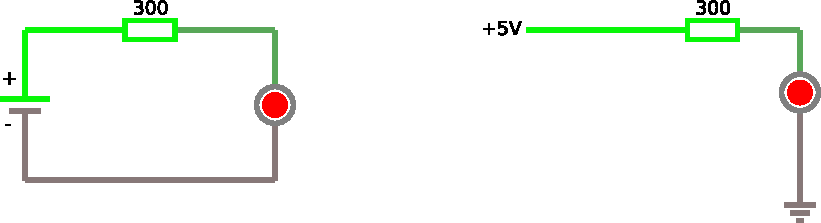
\includegraphics[width=\textwidth]{2-hardwaredesign/img/mini-stromkreis}
    \end{center}

    \hfill%
    \CircuitJS{https://www.falstad.com/circuit/circuitjs.html?ctz=CQAgjCAMB0l3BWcMBMcUHYMGZIA4UA2ATmIxAUgoqoQFMBaMMAKADcQ9CAWCwqrr248ooytSqToCFgCdOI4bzCQUQkVVyQWAd2Rq+AkQn5QWYQin3rlq3iapWAJnQBmAQwCuAGwAuDbzoncFEpSFYAJXA1PBAlcAtY+Mk42lCoaTlo7iSRMGxTZJAtc0twAqp4-NMEbl5nNy8-AKCQlJhwlgBzcpq63toMQlCWAA9ObmI40k4EKcorZSsAHQAHMdmIBBRYvAQkBGwIJZAGFiA}
    \bigskip

    \parbox{\linewidth}{
        \scriptsize

        Elektrische Schaltungen werden immer als \textbf{Stromkreis} entworfen
        und in einem \textbf{Schaltplan} dokumentiert. Gedanklich fließt der
        Strom in diesem vom Pluspol zum Minuspol (linke, eher seltene Darstellung)
        bzw. vom Pluspol der Spannungsquelle zur Masse (rechte Darstellung).
        Tatsächlich beruht diese Annahme aber auf einem Irrtum, weil es die
        negativ geladenen Elektronen sind, die sich vom Minus- zum Pluspol bewegen.
        Da sich dadurch aber nur das Vorzeichen in den Berechnungen ändert, wurde
        die Konvention unter dem Namen \textbf{technische Stromrichtung} in Abgrenzung
        zur \textbf{tatsächlichen Stromrichtung} beibehalten.
        \smallskip

        Die Symbole im Schaltplan haben folgende Bedeutung:
        \smallskip

        \begin{center}
            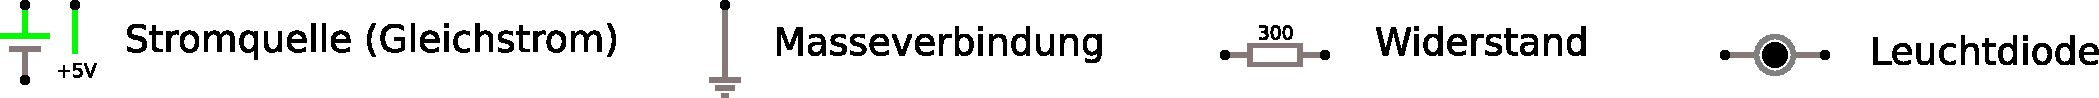
\includegraphics[width=\textwidth]{2-hardwaredesign/img/schaltsymbole}
        \end{center}
    }
\end{frame}

%%% Folie
\begin{frame}[allowframebreaks]{Das Ohmsche Gesetz}
    \begin{columns}
        \column{.4\textwidth}
        \begin{center}
            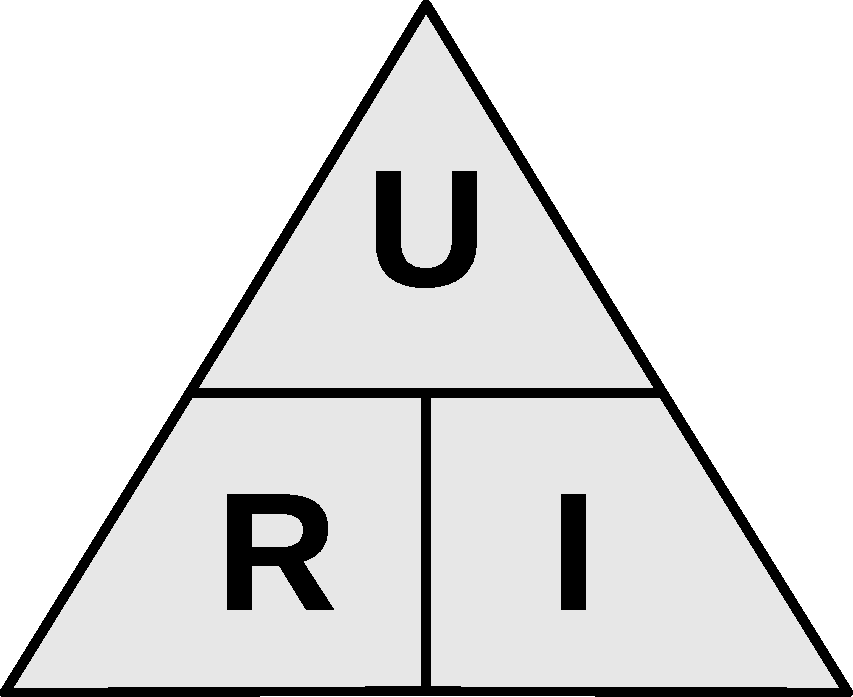
\includegraphics[width=.4\textwidth]{2-hardwaredesign/img/formel_uri}
        \end{center}

        \medskip

        \begin{tabular}{ccll}
            $U$ & = & $R \times I$ & {\scriptsize Spannung in Volt} \\
            $R$ & = & $U / I$ & {\scriptsize Widerstand in Ohm} \\
            $I$ & = & $U / R$ & {\scriptsize Stromstärke in Ampere}\\
        \end{tabular}

        \column{0.6\textwidth}
        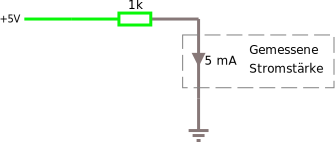
\includegraphics[width=\textwidth]{2-hardwaredesign/img/ohmsches-gesetz-schaltplan}

        \hfill%
        \CircuitJS{https://www.falstad.com/circuit/circuitjs.html?ctz=CQAgjCAMB0l3BWcMBMcUHYMGZIA4UA2ATmIxAUgoqoQFMBaMMAKACURiAWLkbQvCDx4q-QVSpdaUGTAQsATpx58ByDClXjkcFtgxUwkDVvWaegiBJYBzMyAv2uI2SwAe4MCmwPIP5sQ+UoQO4JoA4nQAtnQAzrF0AHZ07p7eDiiaASFcKEi8XiAAygAuCgD2UbElACcKANYpAEbICCHYeAVoglz6UCxAA}
    \end{columns}

    \bigskip

    \Justified{
        \scriptsize

        Die \textbf{Spannung} einer Stromquelle sorgt dafür, dass sich die Elektronen in
        Bewegung setzen und ein Strom fließt, wenn zwischen beiden Polen eine elektrische
        Verbindung hergestellt wird. Die dabei entstehende \textbf{Stromstärke} hängt
        vom \textbf{Widerstand} aller durchlaufenen Bauteile (und dem Innenwiderstand
        der Stromquelle) ab. In bestimmten Fällen kann ein linearer Zusammenhang entsprechend
        der Formel $I = U / R$ angenommen werden, so dass mit zwei bekannten Werten
        der dritte errechnet werden kann.
        \smallskip

        Für uns ist dies besonders wichtig, um die maximale Stromstärke zu begrenzen,
        die der Raspberry Pi an ein angeschlossenes Bauteil abgibt, um sowohl den
        Rasbperry Pi als auch das Bauteil vor Beschädigungen zu schützen. Beispiele
        für typische Fragestellungen sind:

        \begin{itemize}
            \item Welche Stromstärke fließt durch eine Schaltung (wie viel Strom ,,zieht`` die Schaltung)?
            \item Welcher Widerstand wird benötigt, um eine bestimmte Stromstärke zu erhalten?
            \item Liegt die Stromstärke innerhalb der erlaubten Grenzen für den Raspberry Pi und das Bauteil?
        \end{itemize}
    }

    \framebreak

    \textcolor{gray}{
        \tiny
        \textbf{Kennlinie:} Stromstärke in Abhängigkeit zur Spannung, der Widerstand entspricht der Tangentensteigung
    }
    {
        \footnotesize

        \begin{columns}
            \column{.33\textwidth}
            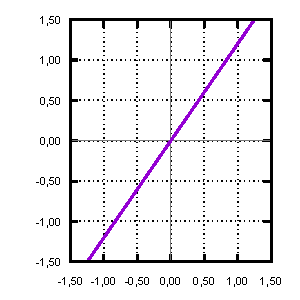
\includegraphics[width=\textwidth]{2-hardwaredesign/img/kennlinie-widerstand} \\
            \smallskip
            \hfill \textbf{Widerstand} \hfill%
            \raisebox{-0.4\height}{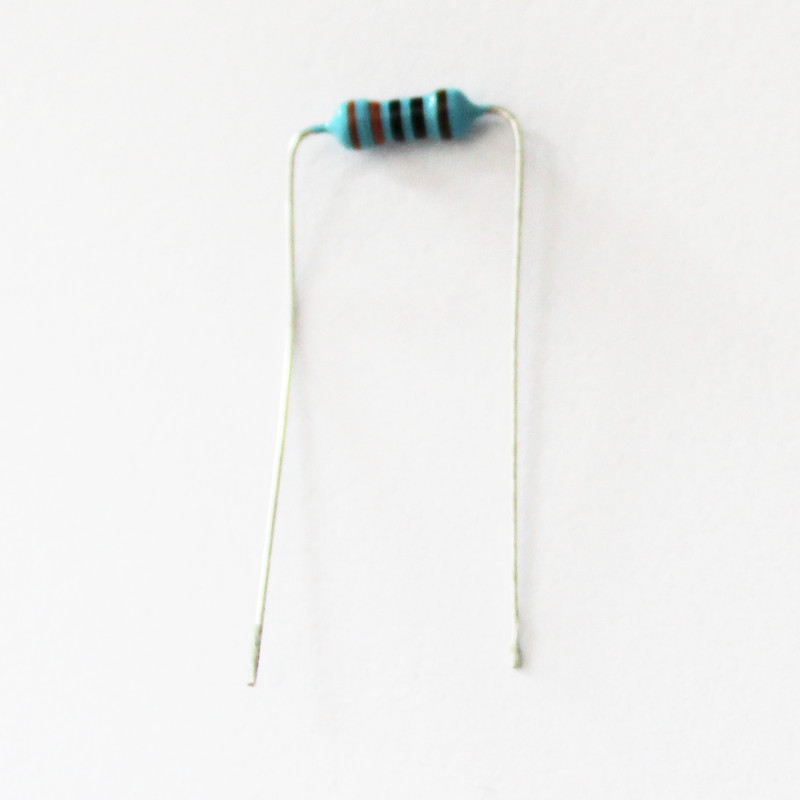
\includegraphics[width=2.5em]{2-hardwaredesign/img/komponenten_elementar_widerstand}}


            \column{.33\textwidth}
            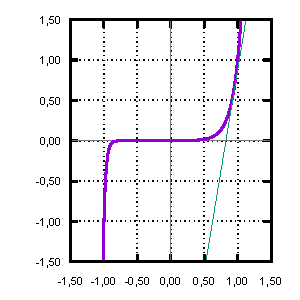
\includegraphics[width=\textwidth]{2-hardwaredesign/img/kennlinie-diode} \\
            \smallskip
            \hfill \textbf{Leuchtdiode} \hfill%
            \raisebox{-0.4\height}{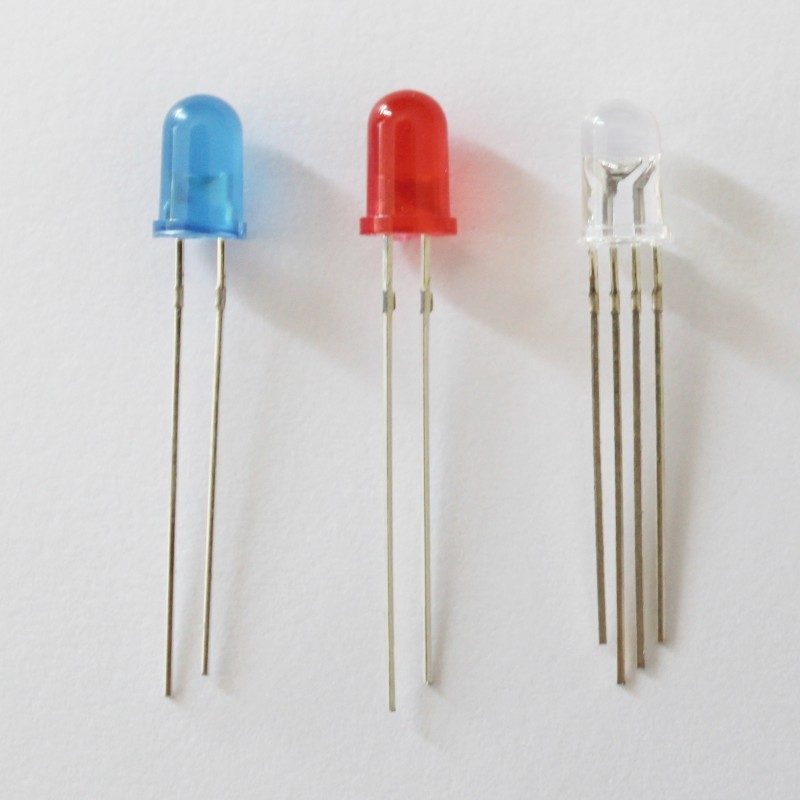
\includegraphics[width=2.5em]{2-hardwaredesign/img/komponenten_elementar_led}}

            \column{.33\textwidth}
            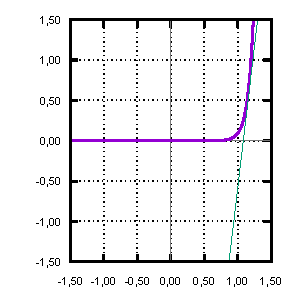
\includegraphics[width=\textwidth]{2-hardwaredesign/img/kennlinie-transistor} \\
            \smallskip
            \hfill \textbf{npn-Transistor} \hfill%
            \raisebox{-0.4\height}{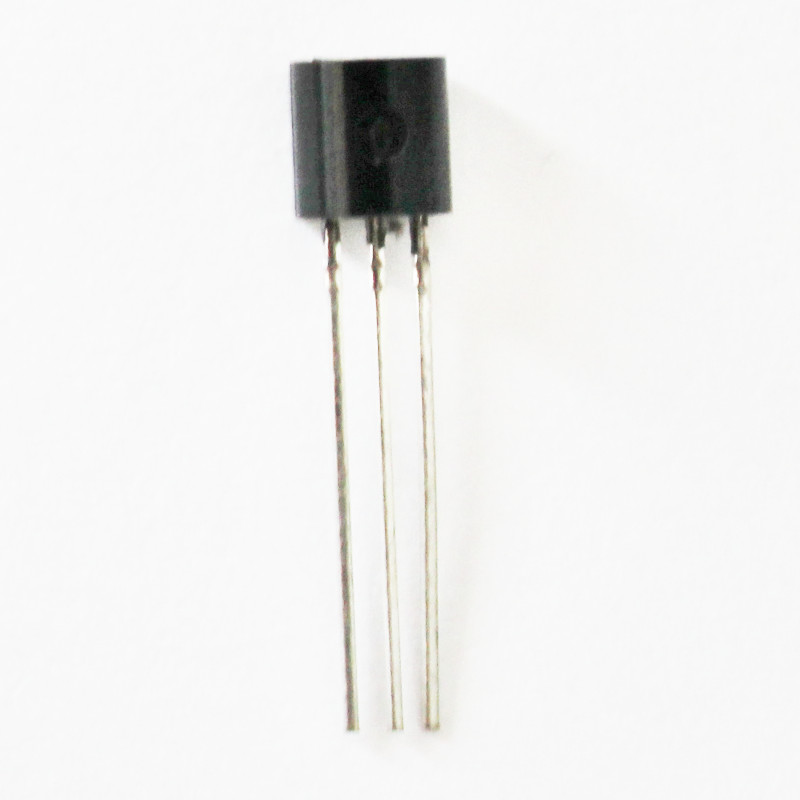
\includegraphics[width=2.5em]{2-hardwaredesign/img/komponenten_elementar_transistor}}
        \end{columns}
    }
    \bigskip

    \Justified{
        \scriptsize

        Das Ohmsche Gesetz gilt nur für \textbf{ideale Widerstände}, die deshalb auch
        \textbf{ohmsche Widerstände} genannt werden. Genau genommen besagt es, dass
        der Widerstand solcher Bauteile für jede Spannung derselbe ist und sich die
        Stromstärke daher linear zur Spannung verhält. In unserem Fall handelt es sich
        dabei um kleine Keramikwiderstände, die wir in unsere Schaltungen einbauen
        (Abbildung links).
        \smallskip

        Insbesondere Bauteile auf Halbleiterbasis besitzen jedoch eine \textbf{nicht-lineare Kennlinie},
        so dass die durchfließende Stromstärke nicht linear von der Spannung abhängt. Der Widerstand
        dieser Bauteile ergibt sich ebenfalls aus Spannung und Stromstärke, besitzt aber keinen konstanten
        Wert. In Anlehnung an das Ohmsche Gesetz kann er näherungsweise als \textbf{differentieller
        Widerstand} $r = \Delta U / \Delta I$ berechnet werden (sog. Kleinsignalverhalten).
    }
\end{frame}

%%% Folie
\begin{frame}{Berechnung der Leistung}
    \begin{columns}
        \column{.4\textwidth}
        \begin{center}
            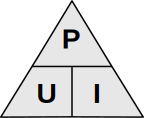
\includegraphics[width=.4\textwidth]{2-hardwaredesign/img/formel_pui}
        \end{center}

        \column{.6\textwidth}
        \begin{tabular}{ccll}
            $P$ & = & $U \times I$ & {\scriptsize Leistung in Watt} \\
            $U$ & = & $P / I$ & {\scriptsize Spannung in Volt} \\
            $I$ & = & $P / U$ & {\scriptsize Stromstärke in Ampere}\\
        \end{tabular}
    \end{columns}

    \vskip 1cm

    \Justified{
        \scriptsize
        Ein weiterer, gelegentlich anzutreffender Begriff ist die in \textbf{Watt}
        gemessene \textbf{Leistung}, welche die innerhalb einer Zeitspanne umgesetzte
        Energie (beispielsweise durch Abwärme) oder die zur Ausführung von Arbeiten
        verfügbare Energie bezeichnet. Ihre elektrische Definition lautet $P = U \times I$,
        so dass ein Watt der Leistung entspricht, die benötigt wird, um an einem
        ohmschen Widerstand von einem Ohm eine Spannung von einem Volt (und damit
        eine Stromstärke von einem Ampere) während einer Sekunde zu erhalten. Daraus
        folgt, dass sich die Leistung aus dem Produkt der beiden anderen Werte
        \textit{Spannung} und \textit{Stromstärke} bildet.
        \smallskip

        Meist kommen wir damit nur in Berührung, wenn es um die \textbf{Nennleistung
        eines Netzteils} oder die damit verbundenen \textbf{Stromkosten} geht. Denn
        anstatt der maximal abgebbaren Stromstärke in Ampere geben die meisten Netzteile
        lediglich eine Maximalleistung in Watt an, die zunächst in Ampere umgerechnet werden muss.
        Typische Fragestellungen könnten dabei sein:
        \smallskip

        \begin{itemize}
            \item Wie viel Leistung steht zum Verrichten anderer Arbeiten zur Verfügung?
            \item Welche maximale Stromstärke kann mein Netzteil bereitstellen?
            \item Wie hoch sind die Stromkosten für die beanspruchte Leistung?
        \end{itemize}
    }
\end{frame}

%-------------------------------------------------------------------------------
\section{Stromversorgung für den Pi}
%-------------------------------------------------------------------------------

%%% Folie
\begin{frame}{Gleichstrom vs. Wechselstrom}
    Grundsätzlich werden drei Arten von Strom unterschieden:
    \medskip

    \begin{block}{Gleichstrom}
        \smallskip
        \parbox{\linewidth}{
            \footnotesize
            Besitzt eine feste Spannung und damit auch feste Polung. \\
            \textbf{Beispiel:} Stromversorgung eines Computers
        }
    \end{block}

    \begin{block}{Wechselstrom}
        \smallskip
        \parbox{\linewidth}{
            \footnotesize
            Die Spannung und damit die auch Polung pendeln gleichmäßig um das
            Massepotential. \\
            \textbf{Beispiel:} Netzstrom aus der Steckdose, analoge Audiosignale
        }
    \end{block}

    \begin{block}{Mischstrom}
        \smallskip
        \parbox{\linewidth}{
            \footnotesize
            Setzt sich aus einem Gleichstrom- und einem Wechselstromanteil zusammen. \\
            \textbf{Beispiel:} Analoge Sensorsignale
        }
    \end{block}

    \bigskip

    \begin{columns}
        \column{.33\textwidth}
        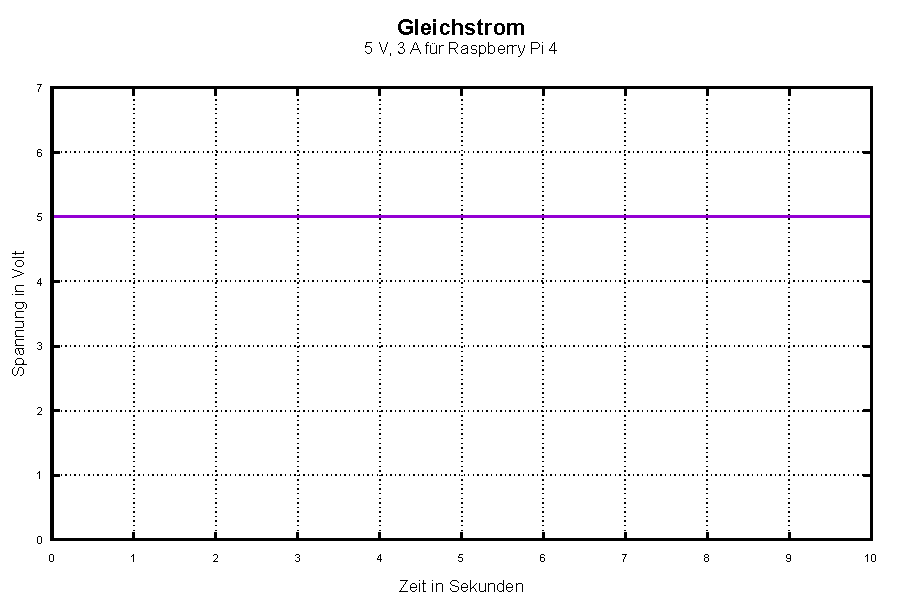
\includegraphics[width=\textwidth]{2-hardwaredesign/img/strom-gleichstrom}

        \column{.33\textwidth}
        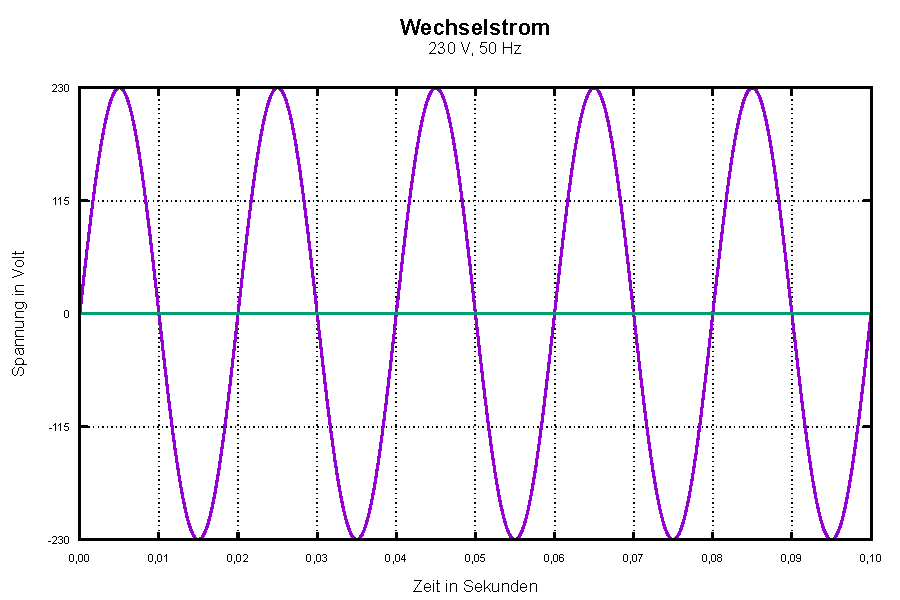
\includegraphics[width=\textwidth]{2-hardwaredesign/img/strom-wechselstrom}

        \column{.33\textwidth}
        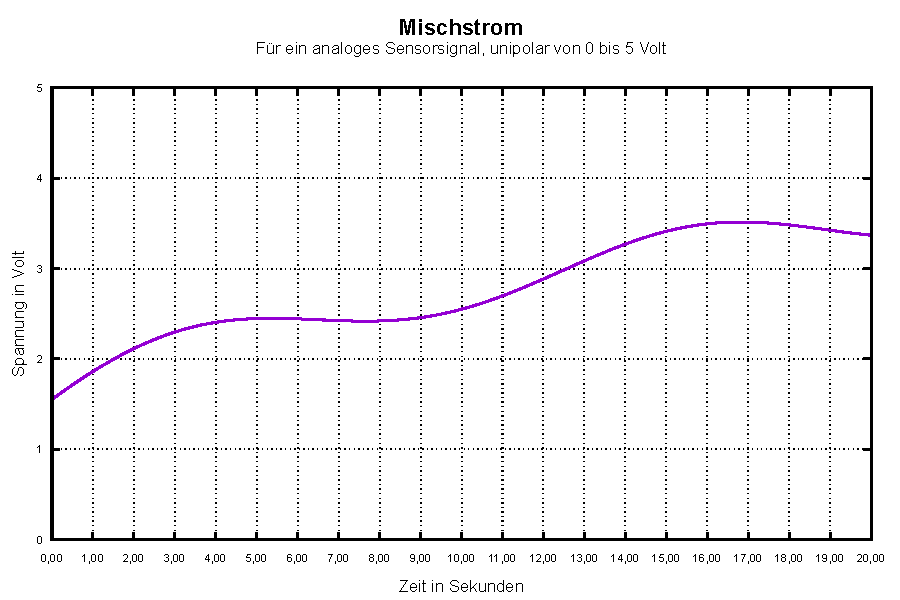
\includegraphics[width=\textwidth]{2-hardwaredesign/img/strom-analogsensor}
    \end{columns}
\end{frame}

%%% Folie
{
\scriptsize

\begin{frame}{Anforderungen des Raspberry Pi}
    \begin{columns}
        \column{.5\textwidth}
        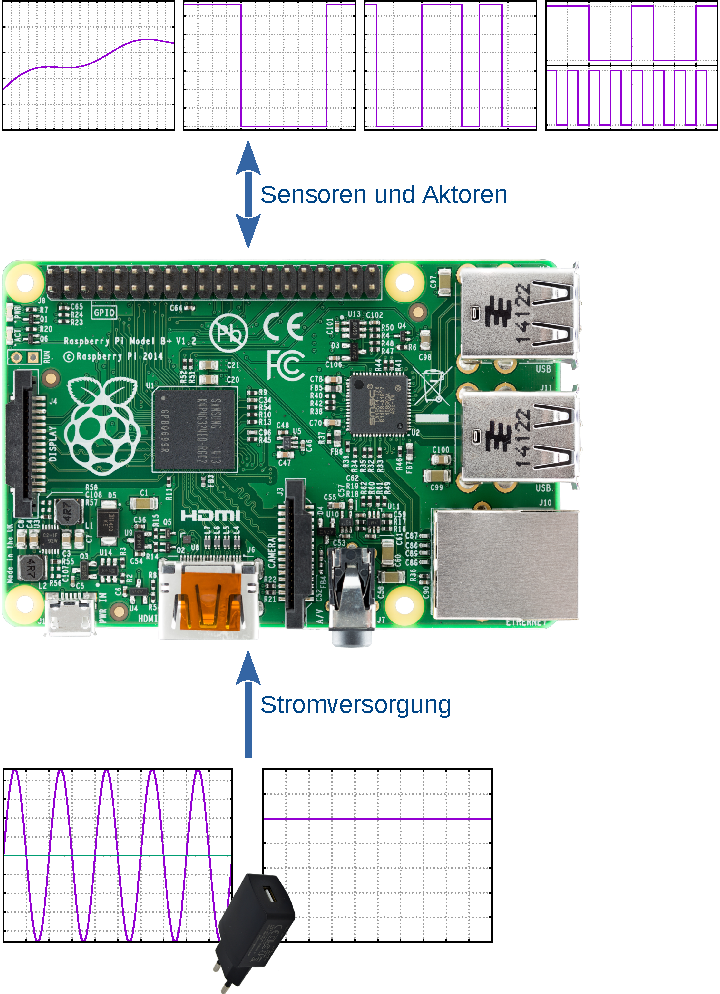
\includegraphics[width=\textwidth]{2-hardwaredesign/img/raspi-stromarten}

        \column{.5\textwidth}

        \begin{block}{Stromversorgung}
            \smallskip
            \parbox{\linewidth}{
                Das Stromnetz liefert Wechselstrom mit 230\,V und 16\,A.
                Der Raspberry Pi benötigt aber \textbf{5\,V Gleichstrom und $\pm$ 3\,A}.
                Das Netzteil muss daher den die Spannung reduzieren und den Strom gleichrichten.
                Eine mobile Stromversorgung muss mindestens genauso viel Strom liefern.
                \smallskip

                \textcolor{red}{
                    Die Spannung muss dabei möglichst konstant sein und darf nicht
                    überschritten werden, um Beschädigungen zu vermeiden!
                }
            }
        \end{block}

        \vfill

        \begin{block}{Batterielaufzeit}
            \smallskip
            \parbox{\linewidth}{
                Kann über die Nennladung der Batterie abgeschätzt werden, wenn diese
                bekannt ist:
                \smallskip

                $\text{Laufzeit in Stunden} = \frac{\text{Nennladung in Ah}}{\text{Stromverbrauch in A}}$
            }
        \end{block}

        \vfill

        \begin{block}{Stromkosten}
            \smallskip
            \parbox{\linewidth}{
                Kann durch Umrechnen des Stromverbrauchs in Killowatt berechnet werden:
                \smallskip

                $\text{Kosten} = \frac{5\,V \times 3\,A}{1000} \times \text{Stunden} \times \text{Strompreis je kWh}$
            }
        \end{block}
    \end{columns}
\end{frame}
}

%-------------------------------------------------------------------------------
\section{Signale verarbeiten und erzeugen}
%-------------------------------------------------------------------------------

%%% Folie
{
    \setbeamertemplate{background canvas}{
        \includegraphics[height=\paperheight, width=\paperwidth]{2-hardwaredesign/img/bauteile}
    }

    \begin{frame}[plain]
    \end{frame}
}

%%% Folie
{
\small

\begin{frame}{Beispiel: Elementare Bauteile}
    \begin{columns}
        \column[b]{.25\textwidth}
        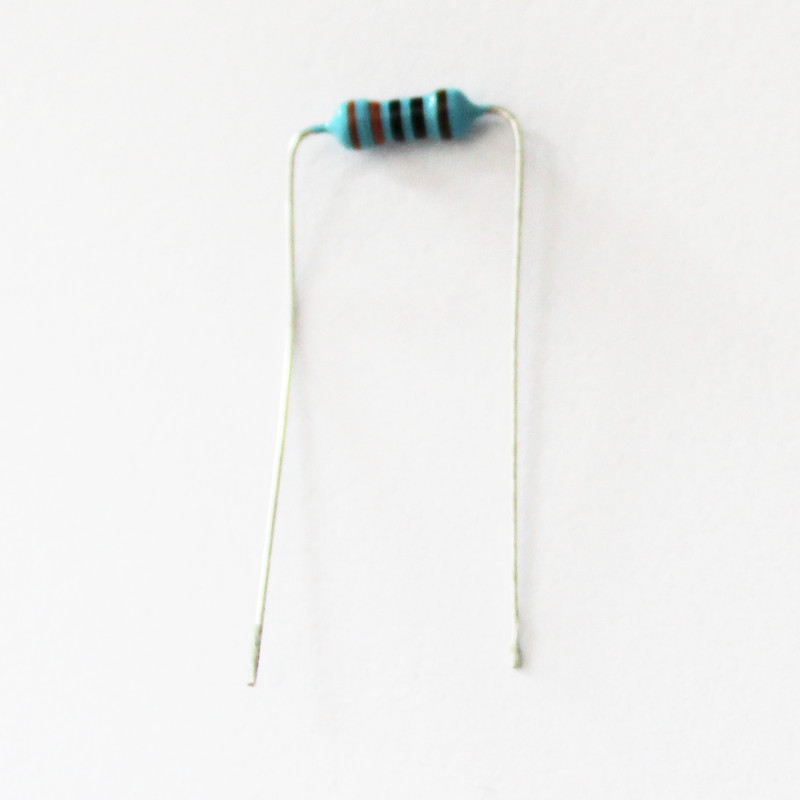
\includegraphics[width=.8\textwidth]{2-hardwaredesign/img/komponenten_elementar_widerstand} \\
        Widerstand

        \column[b]{.25\textwidth}
        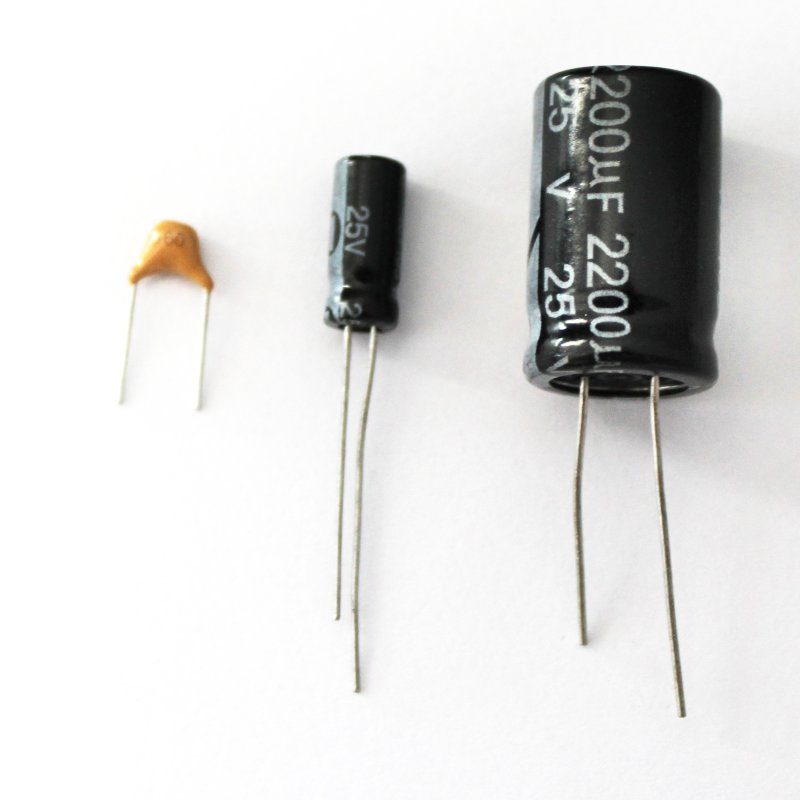
\includegraphics[width=.8\textwidth]{2-hardwaredesign/img/komponenten_elementar_kondensator} \\
        Kondensator

        \column[b]{.25\textwidth}
        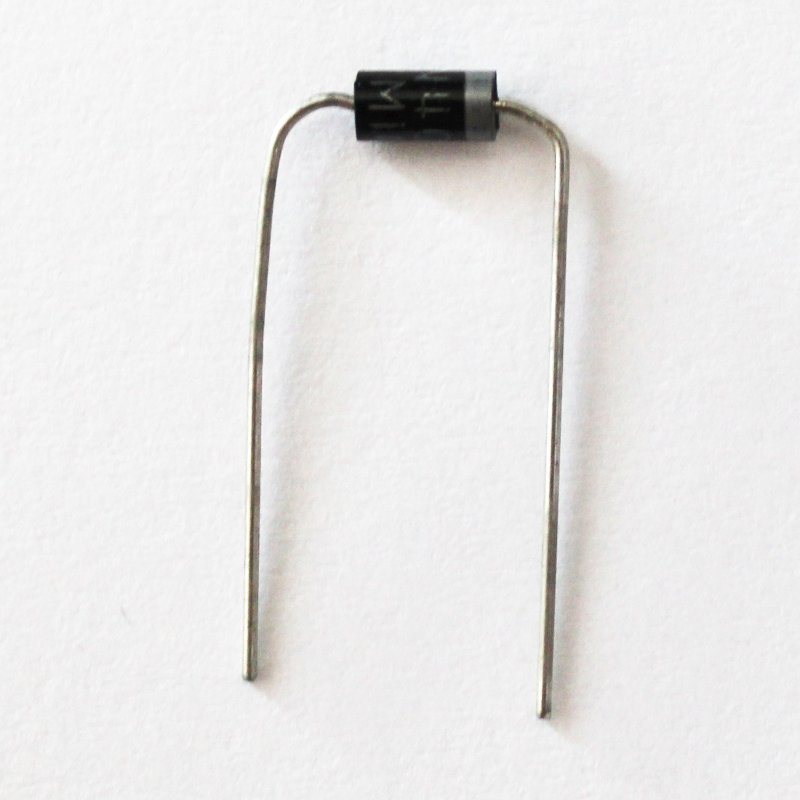
\includegraphics[width=.8\textwidth]{2-hardwaredesign/img/komponenten_elementar_diode} \\
        Diode

        \column[b]{.25\textwidth}
        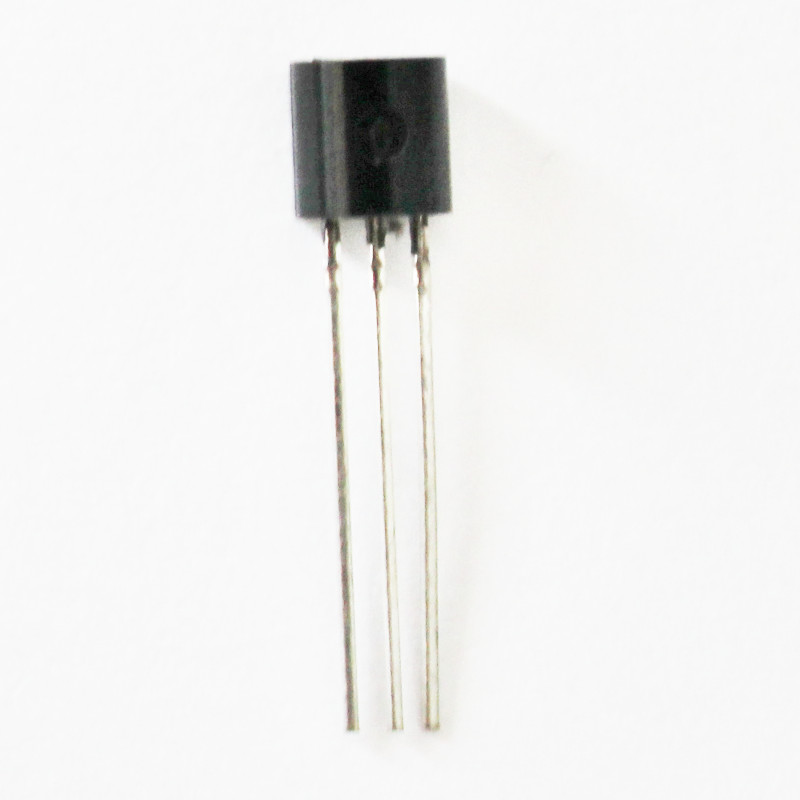
\includegraphics[width=.8\textwidth]{2-hardwaredesign/img/komponenten_elementar_transistor} \\
        Transistor
    \end{columns}

    \bigskip

    \begin{columns}
        \column[b]{.25\textwidth}
        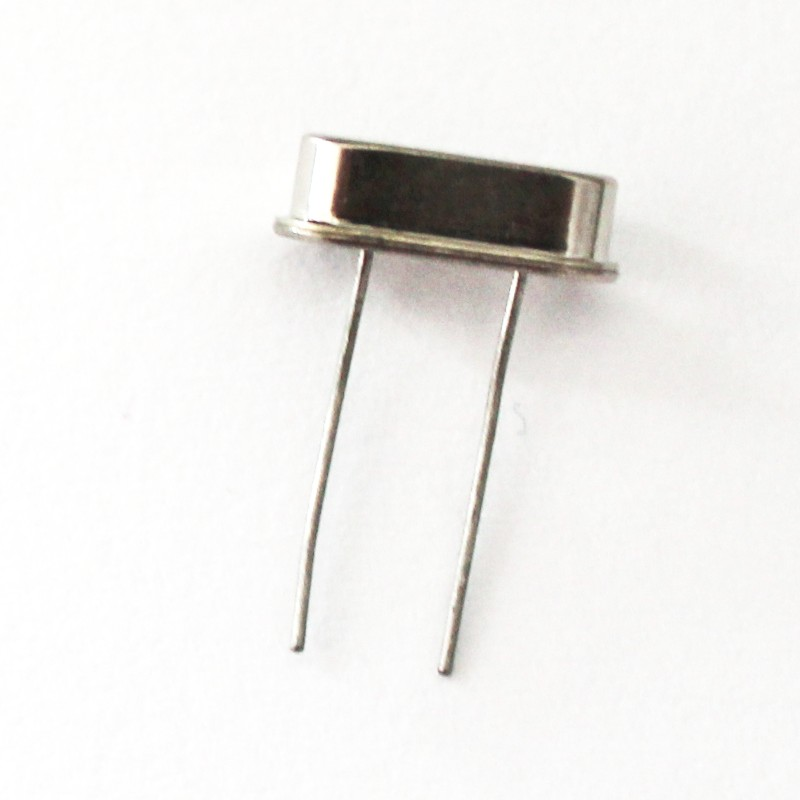
\includegraphics[width=.8\textwidth]{2-hardwaredesign/img/komponenten_elementar_quartz} \\
        Quartz-Kristal

        \column[b]{.25\textwidth}
        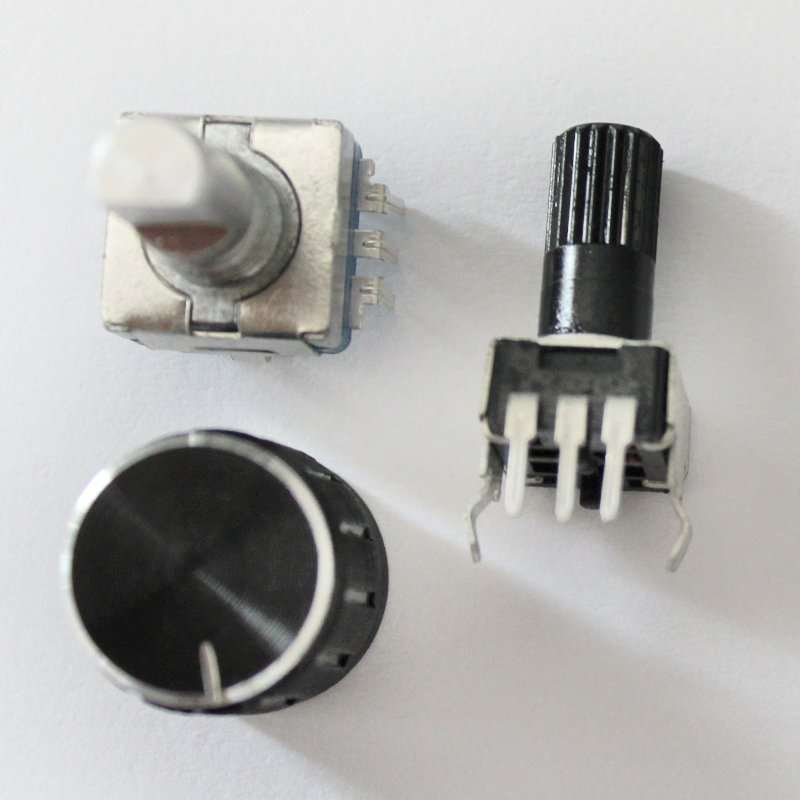
\includegraphics[width=.8\textwidth]{2-hardwaredesign/img/komponenten_elementar_drehregler} \\
        Drehregler

        \column[b]{.25\textwidth}
        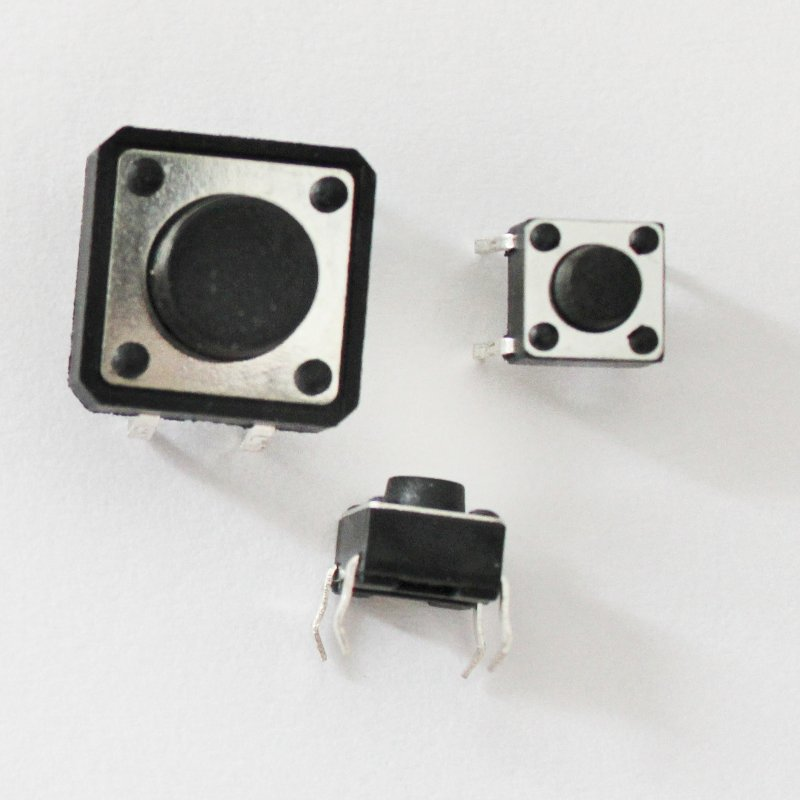
\includegraphics[width=.8\textwidth]{2-hardwaredesign/img/komponenten_elementar_taster} \\
        Taster, Schalter

        \column[b]{.25\textwidth}
        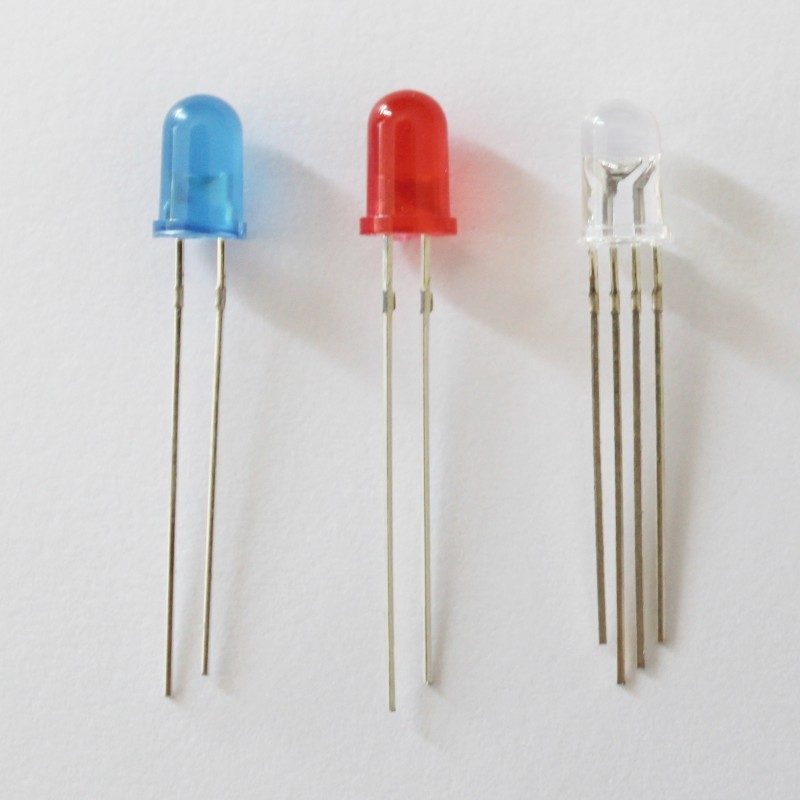
\includegraphics[width=.8\textwidth]{2-hardwaredesign/img/komponenten_elementar_led} \\
        Leuchtdiode
    \end{columns}
\end{frame}
}

%%% Folie
{
\small

\begin{frame}{Beispiel: Integrierte Schaltkreise}
    \begin{columns}
        \column[b]{.5\textwidth}
        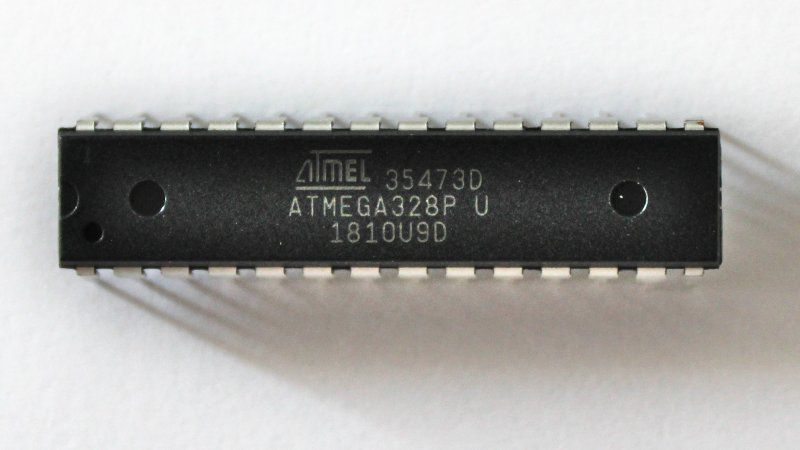
\includegraphics[width=.8\textwidth]{2-hardwaredesign/img/komponenten_ic_prozessor} \\
        Mikroprozessor, Mikrocontroller

        \column[b]{.5\textwidth}
        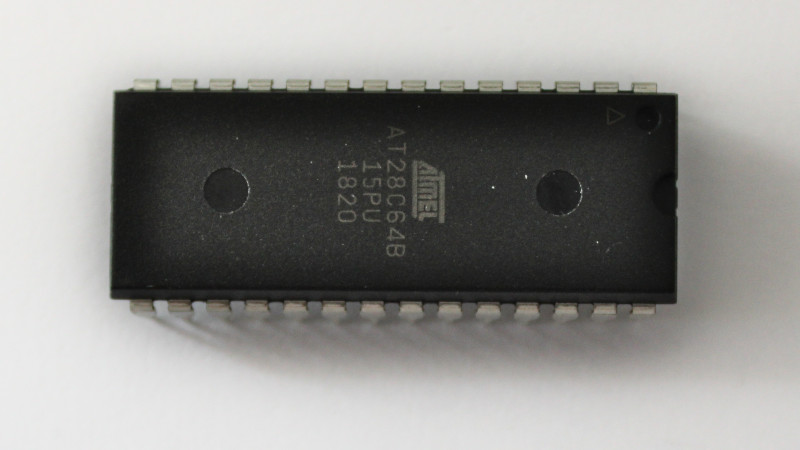
\includegraphics[width=.8\textwidth]{2-hardwaredesign/img/komponenten_ic_speicher} \\
        Speicherbaustein
    \end{columns}

    \bigskip

    \begin{columns}
        \column[b]{.5\textwidth}
        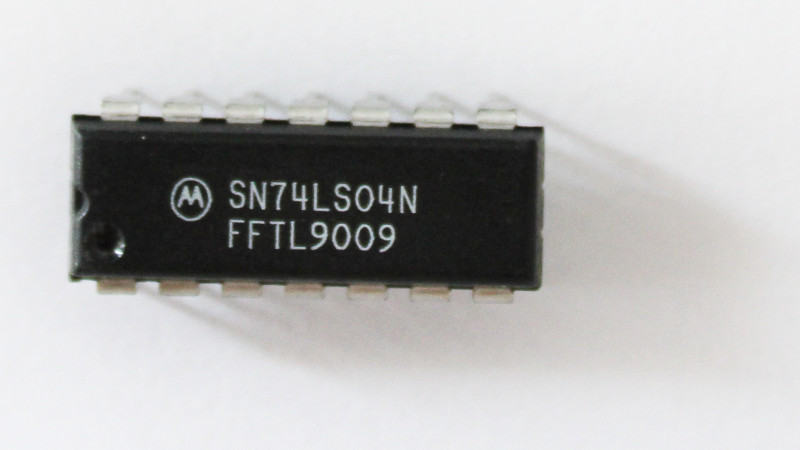
\includegraphics[width=.8\textwidth]{2-hardwaredesign/img/komponenten_ic_logikgatter} \\
        Logikbaustein (AND, OR, XOR, ...)

        \column[b]{.5\textwidth}
        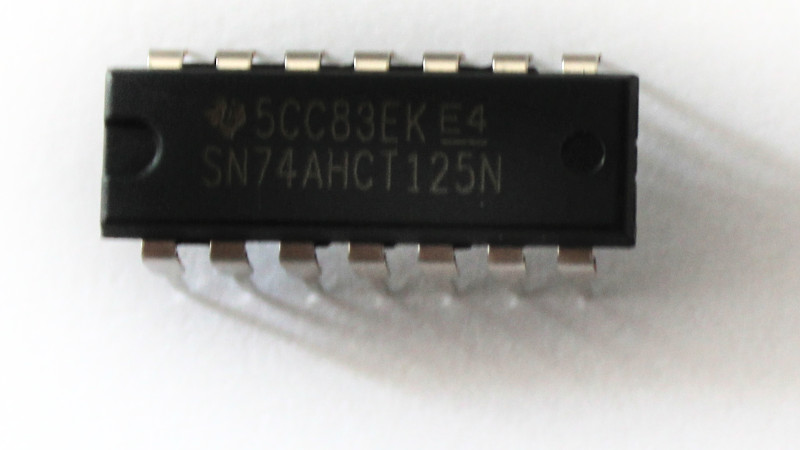
\includegraphics[width=.8\textwidth]{2-hardwaredesign/img/komponenten_ic_levelshifter} \\
        Level Shifter
    \end{columns}
\end{frame}
}

%%% Folie
{
\small

\begin{frame}{Beispiel: Vorgefertigte Baugruppen}
    \begin{columns}
        \column[b]{.5\textwidth}
        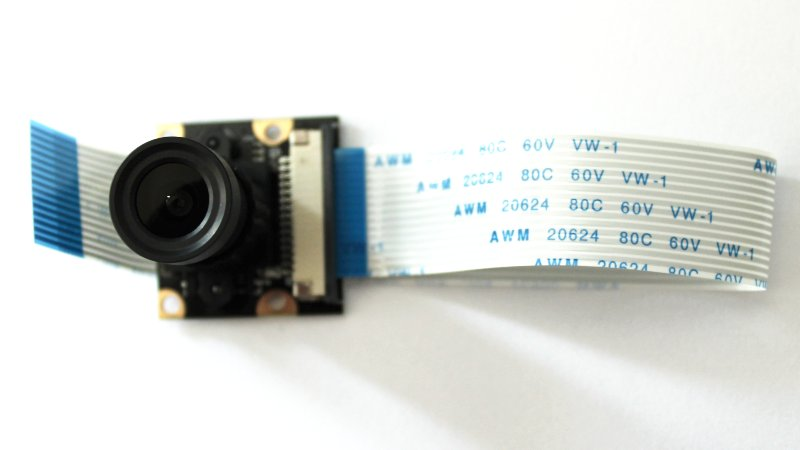
\includegraphics[width=.8\textwidth]{2-hardwaredesign/img/komponenten_baugruppen_kamera} \\
        Kameramodul

        \column[b]{.5\textwidth}
        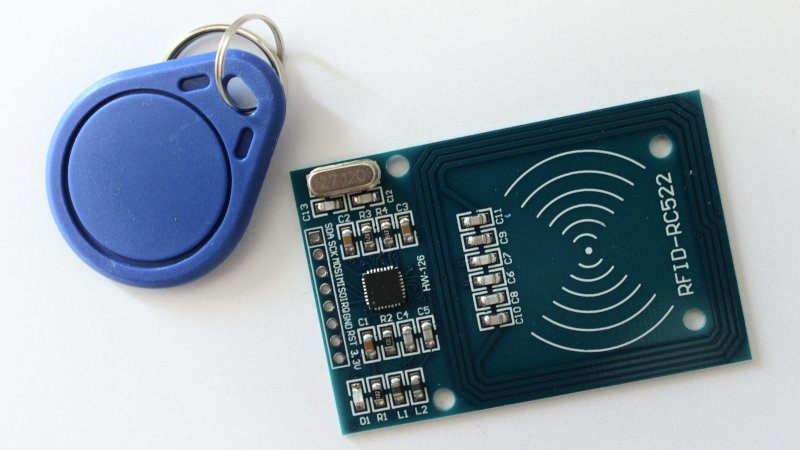
\includegraphics[width=.8\textwidth]{2-hardwaredesign/img/komponenten_baugruppen_rfid} \\
        RFID-Leser
    \end{columns}

    \bigskip

    \begin{columns}
        \column[b]{.5\textwidth}
        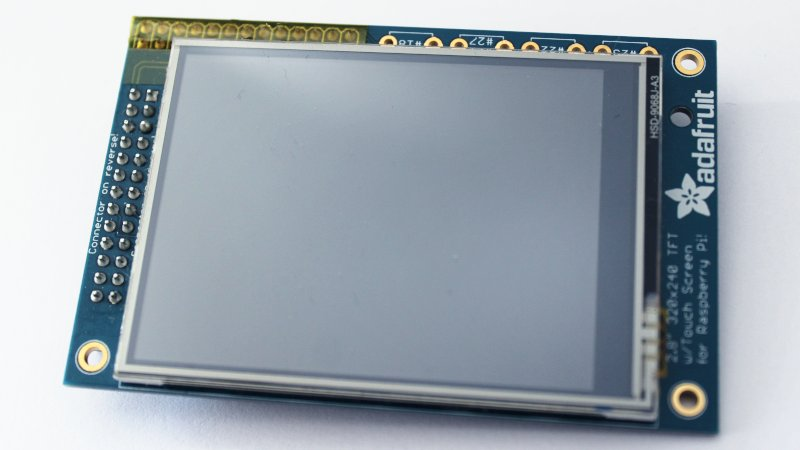
\includegraphics[width=.8\textwidth]{2-hardwaredesign/img/komponenten_baugruppen_display} \\
        Display

        \column[b]{.5\textwidth}
        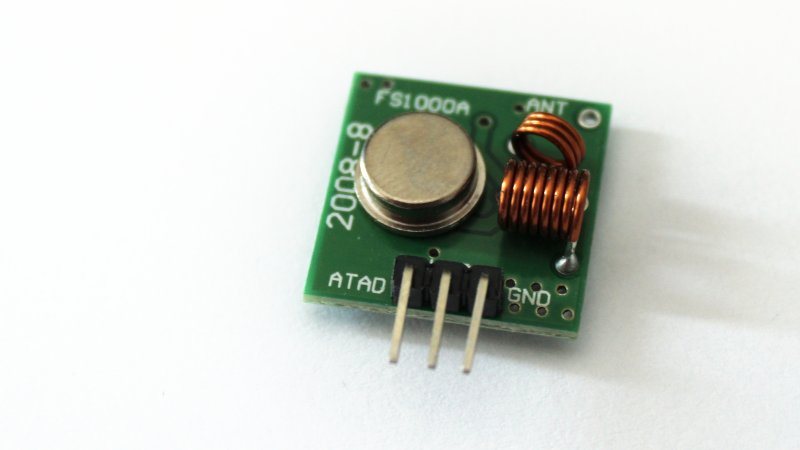
\includegraphics[width=.8\textwidth]{2-hardwaredesign/img/komponenten_baugruppen_funk} \\
        Funkmodul
    \end{columns}
\end{frame}
}

%%% Folie
{
\tiny

\begin{frame}[allowframebreaks]{Beispiel: Sensorkit aus der Vorlesung}
    \begin{columns}
        \column{\dimexpr\paperwidth-28pt}
        \begin{center}
            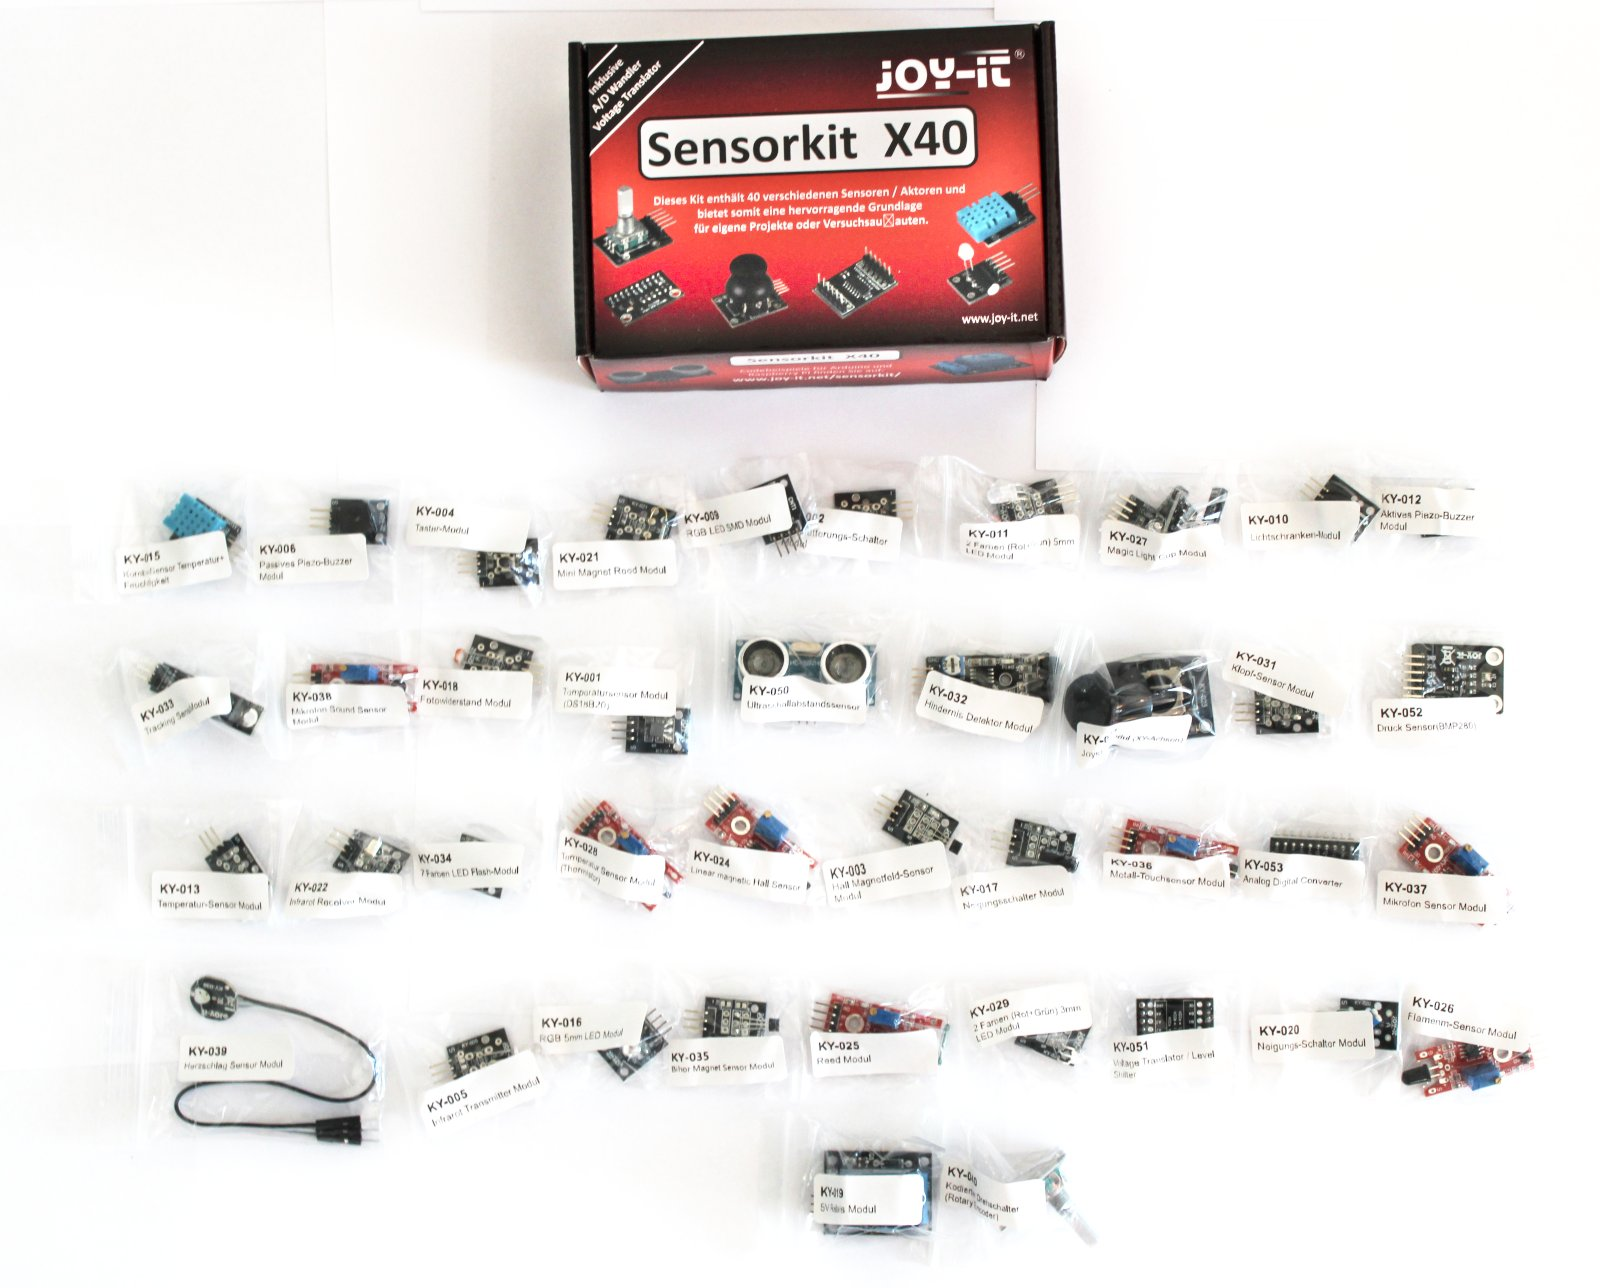
\includegraphics[height=.8\textheight]{2-hardwaredesign/img/sensorkit_alle}
        \end{center}
    \end{columns}

    \begin{block}{Umweltsensoren}
        \medskip
        \begin{columns}
            \column{0.5\textwidth}
            KY-001: Temperatursensor (DS18B20) \\
            KY-002: Erschütterungsschalter \\
            KY-003: Hall Magnetfeldsensor \\
            KY-010: Lichtschranke \\
            KY-013: Temperatursensor \\
            KY-015: Temperatur, Feuchtigkeit (DHT11) \\
            KY-017: Neigungsschalter \\
            KY-018: Fotowiderstand \\
            KY-020: Neigungsschalter \\
            KY-021: Mini Magnet-Reedkontakt \\
            KY-024: Linear Magnetic Hall-Sensor \\
            KY-025: Reedkontakt \\
            KY-026: Flammensensor \\

            \column{0.5\textwidth}
            KY-027: Magic Light Cup  \\
            KY-028: Temperatursensor (Thermistor) \\
            KY-031: Klopfsensor \\
            KY-032: Hindernisdetektor \\
            KY-033: Trackingsensor \\
            KY-035: Bihor Magnetsensor \\
            KY-036: Metall-Touchsensor \\
            KY-037: Mikrofon Soundsensor \\
            KY-038: Mikrofon Soundsensor \\
            KY-039: Herzschlagsensor \\
            KY-050: Ultraschallabstandssensor \\
            KY-052: Drucksensor (BMP280) \\
        \end{columns}
    \end{block}

    \begin{block}{Ein-/Ausgabemodule}
        \medskip
        \begin{columns}
            \column{0.5\textwidth}
            KY-004: Taster \\
            KY-022: Infrarot-Receiver \\
            KY-023: XY-Joystick \\
            KY-040: Kodierter Drehschalter (Rotary Encoder) \\
            \smallskip
            KY-005: Infrarot-Transmitter \\
            KY-006: Passiver Piezo-Buzzer \\
            KY-009: RGB-LED (Surface-Mount) \\

            \column{0.5\textwidth}
            KY-011: 2-Farben (Rot und Grün) LED \\
            KY-012: Aktiver Piezo-Buzzer \\
            KY-016: RGB-LED (Through-Hole) \\
            KY-019: 5V Relais \\
            KY-029: 2-Farben (Rot und Grün) LED \\
            KY-034: 7-Farben LED \\
        \end{columns}
    \end{block}

    \begin{block}{Hilfsbausteine}
        \medskip
        \begin{columns}
            \column{0.5\textwidth}
            KY-051: Voltage Translator / Level Shifter \\

            \column{0.5\textwidth}
            KY-053: Analog/Digital Converter \\
        \end{columns}
    \end{block}
\end{frame}
}

%%% Folie
{
\small

\begin{frame}{Beispiel: Modular einsetzbare Geräte}
    \begin{columns}
        \column[b]{.5\textwidth}
        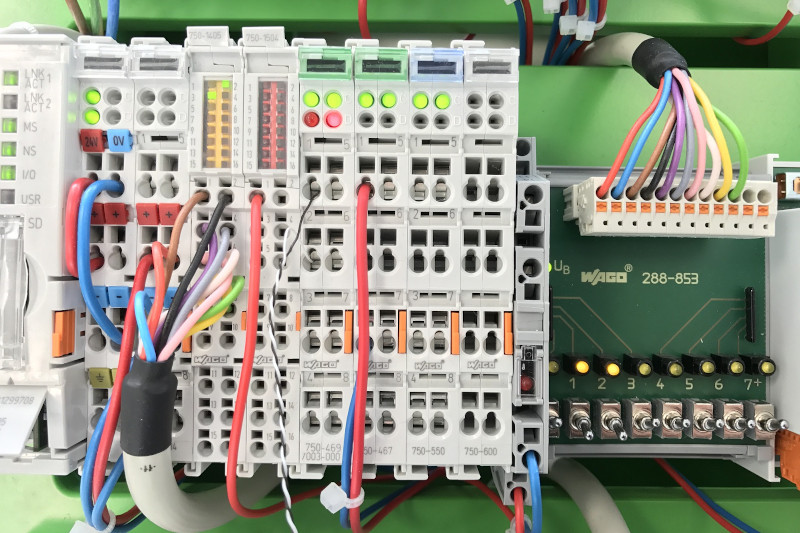
\includegraphics[width=.8\textwidth]{2-hardwaredesign/img/komponenten_geraete_industriesteuerung} \\
        Industrielle Steuergeräte

        \column[b]{.5\textwidth}
        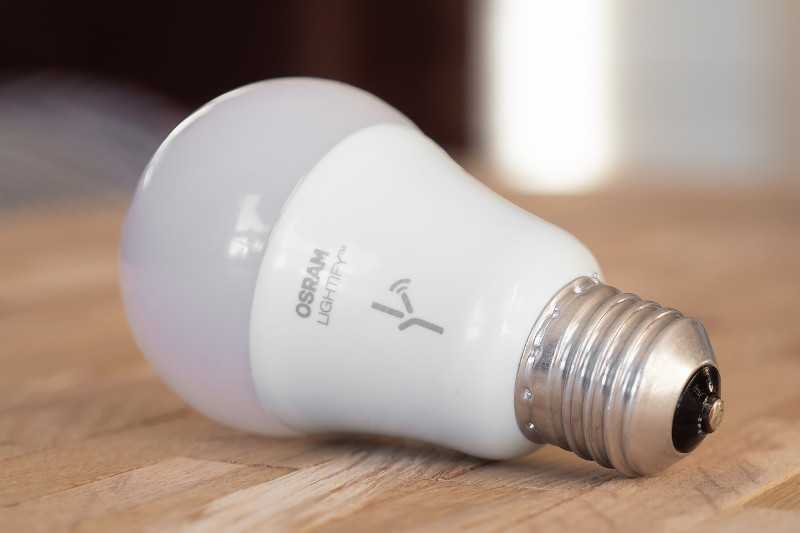
\includegraphics[width=.8\textwidth]{2-hardwaredesign/img/komponenten_geraete_smarthome} \\
        Smart-Home-Komponenten
    \end{columns}

    \bigskip

    \begin{columns}
        \column[b]{.5\textwidth}
        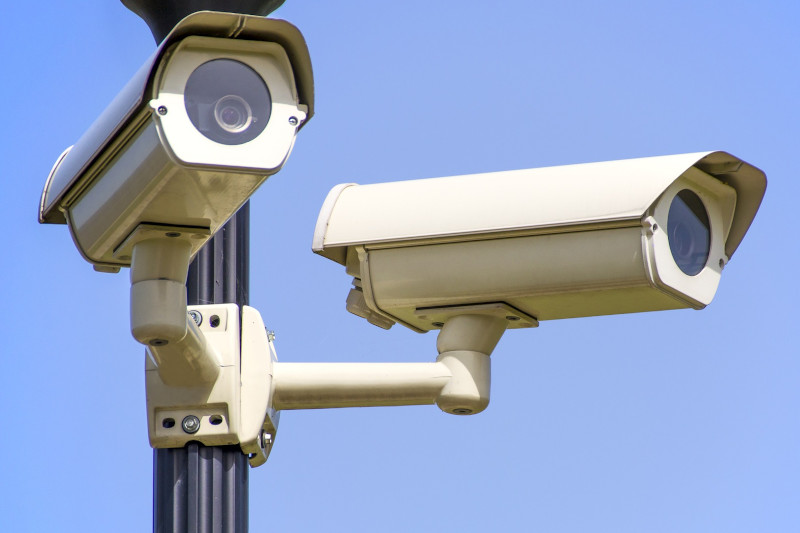
\includegraphics[width=.8\textwidth]{2-hardwaredesign/img/komponenten_geraete_ipkamera} \\
        IP-Kameras

        \column[b]{.5\textwidth}
        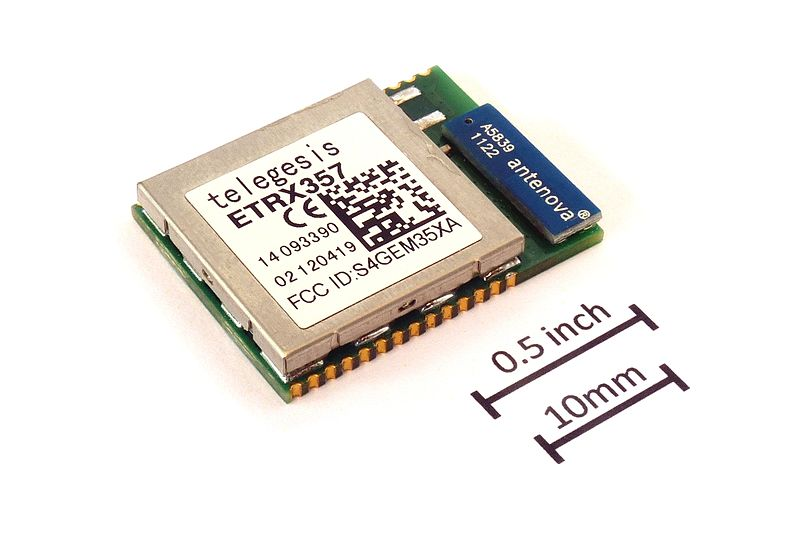
\includegraphics[width=.8\textwidth]{2-hardwaredesign/img/komponenten_geraete_zigbee} \\
        ZigBee-Sensoren und Aktoren
    \end{columns}
\end{frame}
}

%%% Folie
{
    \setbeamertemplate{background canvas}{
        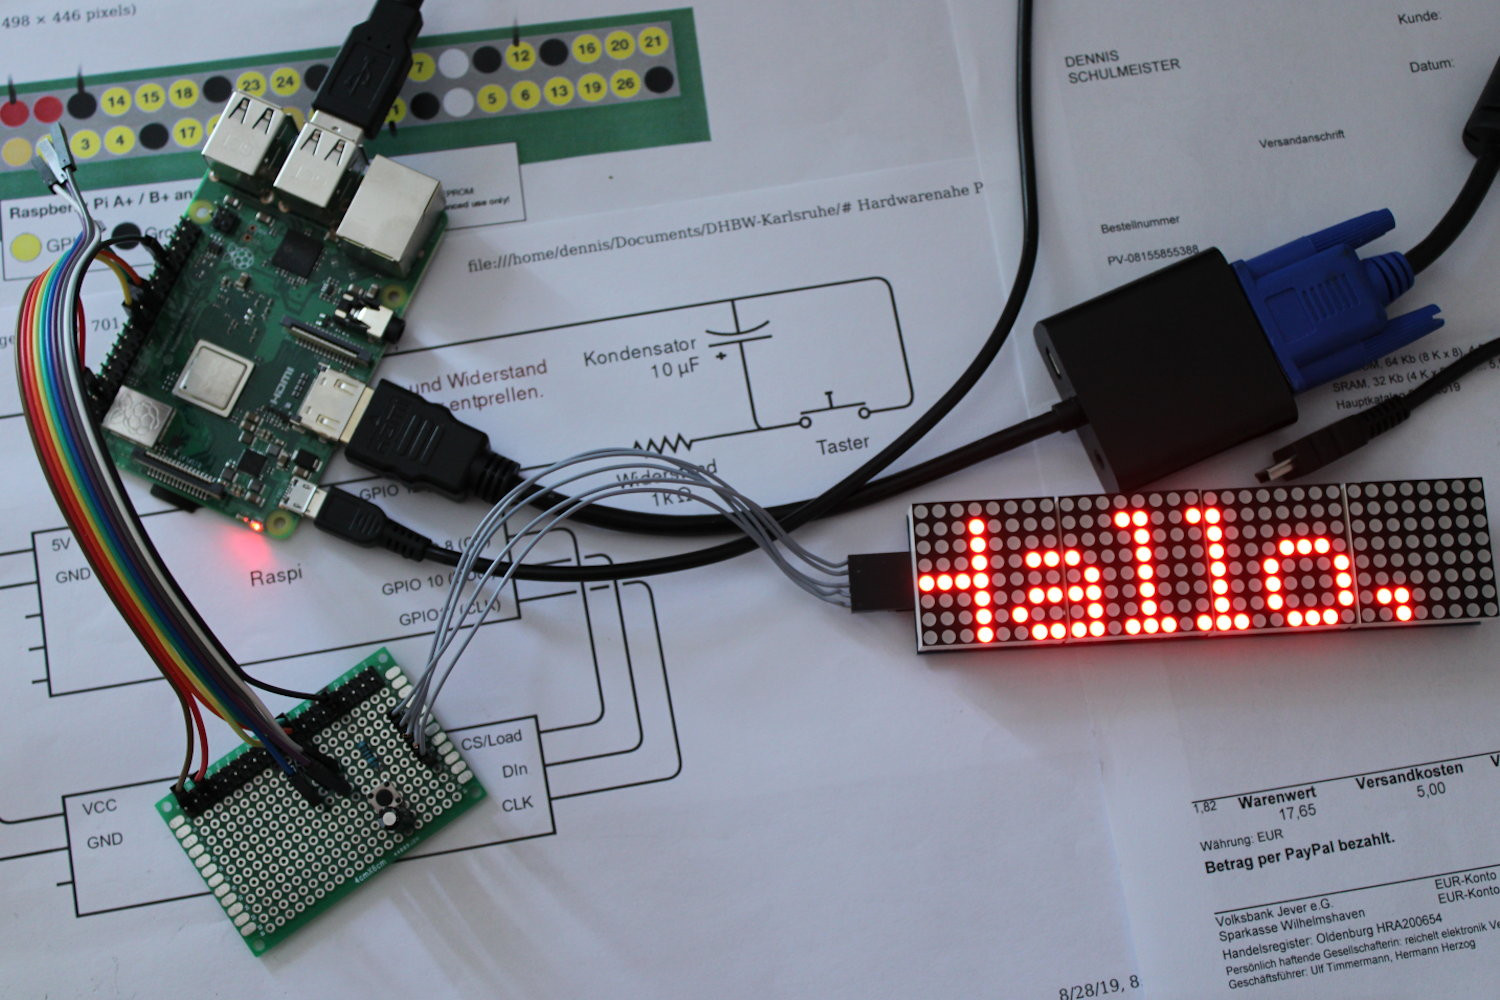
\includegraphics[height=\paperheight, width=\paperwidth]{2-hardwaredesign/img/vorgehen_lochrasterplatine}
    }

    \begin{frame}[plain]
    \end{frame}
}

%%% Folie
\begin{frame}{Häufig vorkommende Signalarten}
        \begin{columns}
        \column[b]{.5\textwidth}
        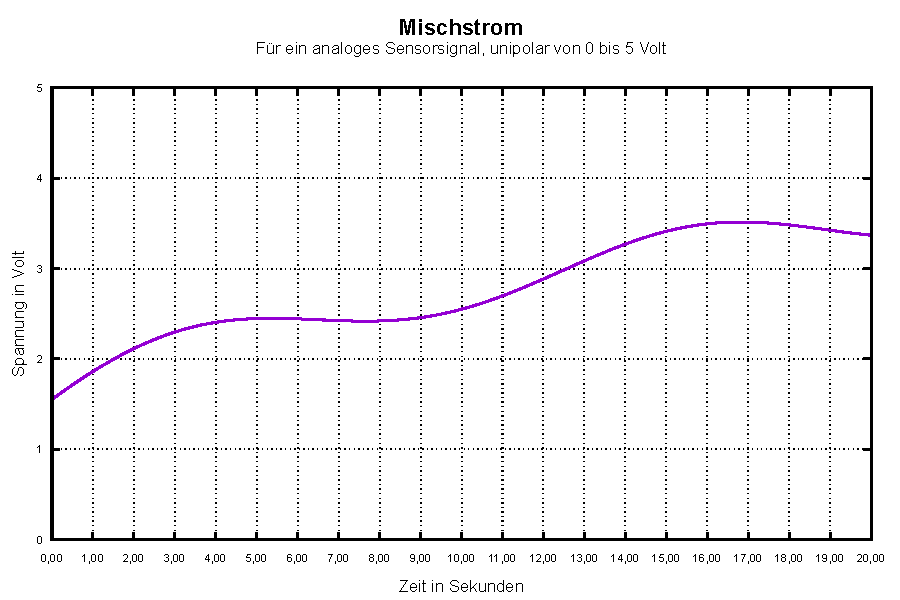
\includegraphics[width=\textwidth]{2-hardwaredesign/img/strom-analogsensor} \\

        \column[b]{.5\textwidth}
        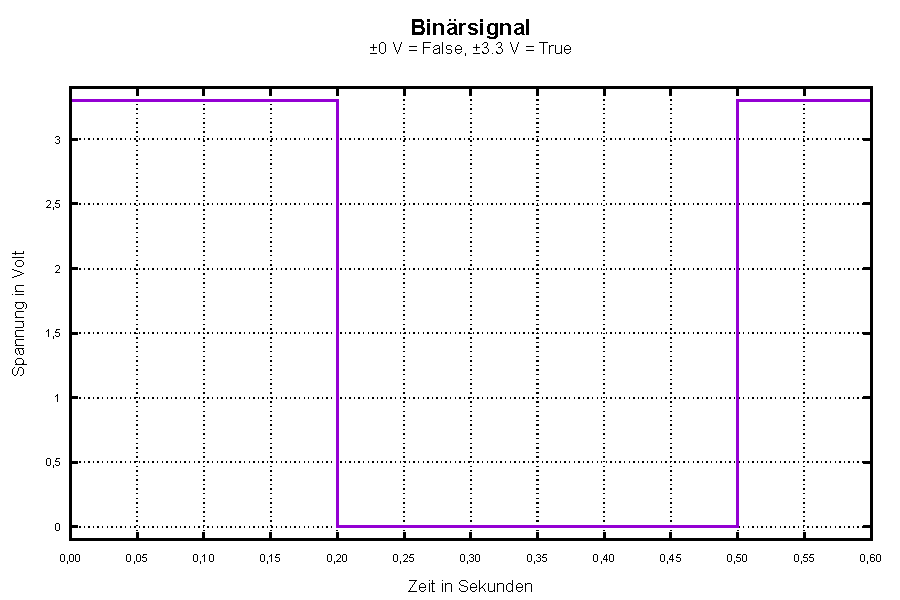
\includegraphics[width=\textwidth]{2-hardwaredesign/img/strom-binary} \\
    \end{columns}

    \bigskip

    \begin{columns}
        \column[b]{.5\textwidth}
        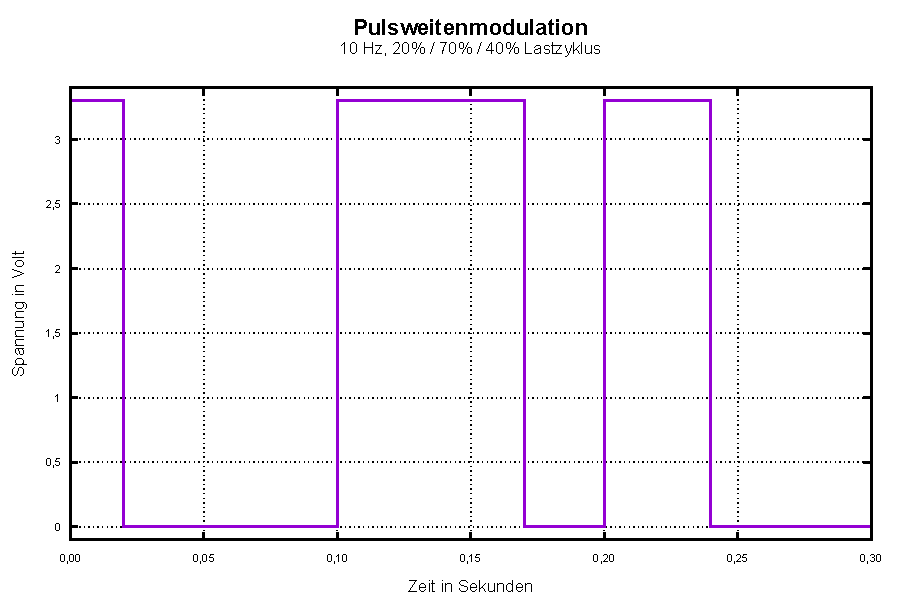
\includegraphics[width=\textwidth]{2-hardwaredesign/img/strom-pwm} \\

        \column[b]{.5\textwidth}
        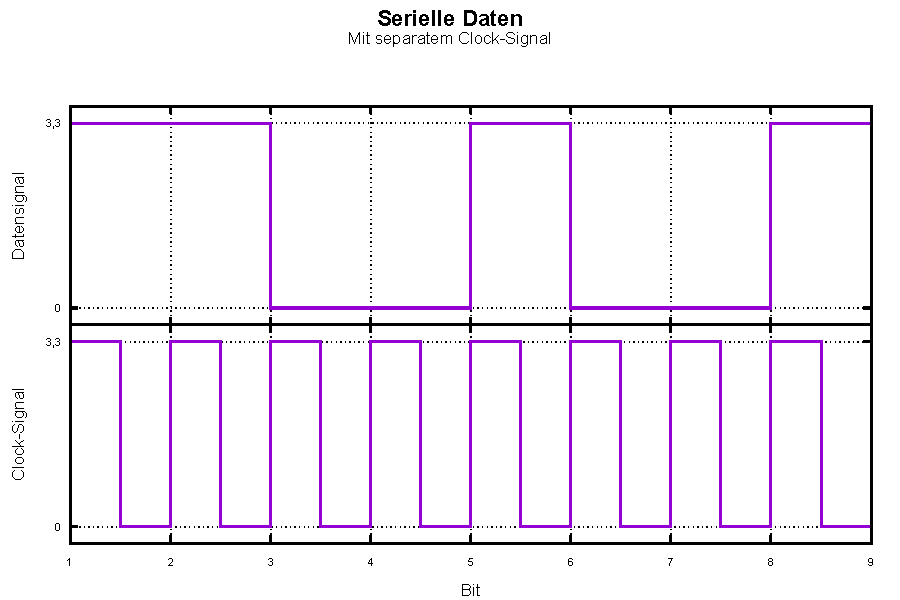
\includegraphics[width=\textwidth]{2-hardwaredesign/img/strom-serial} \\
    \end{columns}
\end{frame}

%%% Folie
\begin{frame}{Anschlüsse am Raspberry Pi}
        \begin{center}
            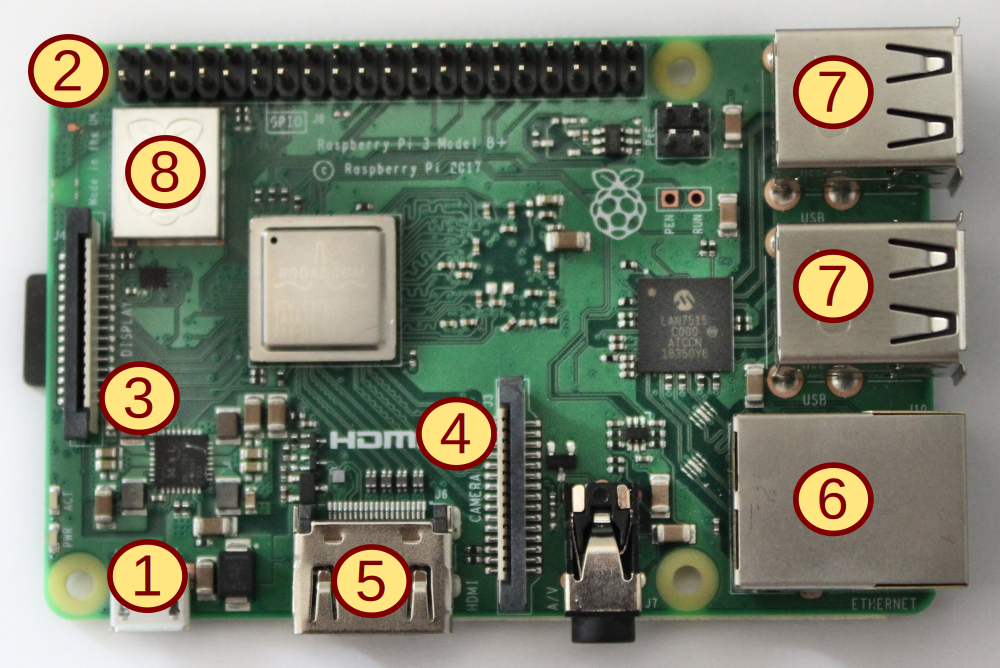
\includegraphics[height=0.5\textheight]{2-hardwaredesign/img/raspberry_anschluesse}
        \end{center}

        \smallskip

        \begin{columns}
            \begin{column}[T]{.5\textwidth}
                \begin{enumerate}
                    \item Mini-USB Stromversorgung
                    \item J8 GPIO-Header
                    \item Display Serial Interface
                    \item Camera Serial Interface
                \end{enumerate}
            \end{column}
            \begin{column}[T]{.5\textwidth}
                \begin{enumerate}
                    \setcounter{enumi}{4}   % Zielwert - 1
                    \item HDMI-Bildschirmanschluss
                    \item LAN-Netzwerkanschluss
                    \item USB (4 Stück)
                    \item WiFi, Bluetooth
                \end{enumerate}
            \end{column}
        \end{columns}
\end{frame}

%%% Folie
{
\footnotesize

\begin{frame}{Der J8 GPIO-Header im Detail}
        \begin{columns}
            \column[b]{.5\textwidth}
            \includegraphics[height=.7\textheight]{2-hardwaredesign/img/pinout}
            %\includegraphics[width=\textwidth]{2-hardwaredesign/img/raspberry_j8}

            \medskip
            \LinkButton{https://pinout.xyz/}{Raspberry Pi Pinout Guide}

            \column[b]{.5\textwidth}
            \begin{block}{Stromquellen}
                \begin{itemize}
                    \item 5V Power
                    \item 3.3V Power
                    \item Ground (Masse)
                \end{itemize}
            \end{block}

            \begin{block}{Digitale Ein-/Ausgänge}
                \begin{itemize}
                    \item GPIO
                    \item Pulsweitenmodulation
                    \item Asynchron serielle Kommunikation
                    \item Synchron serielle Kommunikation \\ (SPI, I²C, I²S, 1-Wire)
                \end{itemize}
            \end{block}

            \begin{alertblock}{Keine analogen Ein-/Ausgänge!}
            \end{alertblock}
        \end{columns}
\end{frame}
}

%%% Folie
{
\footnotesize

\begin{frame}{Bevor es losgehen kann: Maximale Grenzwerte}
    \parbox{\linewidth}{
        Um eine Beschädigung des Raspberry Pi zu vermeiden, müssen folgende Grenzwerte unbedingt
        eingehalten werden. Ggf. müssen daher nach dem Ohmschen Gesetz berechnete Widerstände in
        Serie zu einem Bauteil angeschlossen werden, um die Stromstärke zu begrenzen. Ebenso muss
        die Summe aller zugeführten und entnommenen Ströme betrachtet werden.
    }

    \bigskip
    \renewcommand{\arraystretch}{1.2}

    \begin{tabularx}{\textwidth}{|p{18em}|X|X|}
        \hline
        \textbf{Parameter} & \textbf{Mindestwert} & \textbf{Maximalwert} \\
        \hline

        Betriebsspannung des Pi & 5\,V & 5\,V \\
        \hline

        Stromverbrauch des Pi & 800\,mA (eher mehr) & -- \\
        \hline

        Stromentnahme an den 3.3\,V-Pins & -- & 50\,mA gesamt \\
        \hline

        Stromentnahme an den 5\,V-Pins & -- & 50\,mA gesamt \\
        \hline

        Stromentnahme an einem GPIO-Pin & -- & 16\,mA \\
        \hline

        Stromentnahme an allen GPIO-Pins & -- & 50\,mA gesamt \\
        \hline
    \end{tabularx}

    \bigskip
    \includegraphics[width=.75\textwidth]{2-hardwaredesign/img/stromentnahme-raspi-schaltplan}

    \hfill%
    \CircuitJS{https://www.falstad.com/circuit/circuitjs.html?ctz=CQAgzCAMB0l3BWEBGGAmOaDsWyQBxoBsAnCViApJZdQgKYC0yyAUADIj7JEhr74QWIoP6DqyEADMAhgBsAzvXDQIkVmCzUSAFh18BIXfrBhek6uoDmQkeDO3BYBGihRWAJy48Dg477cqdQAjIRIkNAQkIh0KTX11AHcjPXteYScHdQAPEBiScHwKLDQTEmp9ZFcAJRkFAAdg+g8PAE8AHQUABQBLVlyiBApsVywdCGwkStcAcS6ASQB5RgBBAFcFKxkAOyt+vIReMB1JLCpwVOmQAFk6pU6AChmPAHs17YATAEp9waPICBYZAQPC8K7sF6JTrtACOnUgADVfocAiVRCRJFcABI9KwAC2hcIUYAANGAkblUJATJBXKgxuBIFMULN6ABbegKJTbej7KlHZAFekFMBoVxXADKABdXmyFFKACceADWvNCqEMx30JDQBWwBXUQA}
\end{frame}
}

%%% Folie
{
\scriptsize

\begin{frame}{Binärsignal ausgeben am Beispiel einer LED}
    \Justified{
        Jeder \textbf{GPIO-Pin} kann softwaregesteuert als \textbf{Eingang oder Ausgang} konfiguriert
        werden. Ausgangspins stellen eine Spannung von \textbf{ca. 3,3\,V} zur Verfügung, um eine
        logische Eins zu signalisieren, sowie \textbf{0\,V} (entspricht einer Verbindung gegen Masse)
        für eine logische Null.
        \smallskip

        Der entnommene Strom muss in der Regel durch einen \textbf{Widerstand} begrenzt werden.
        Da die verfügbare Spannung und die gewünschte Stromstärke bekannt sind, kann dieser mit
        dem \textbf{Ohmschen Gesetz} leicht berechnet werden. Dabei muss jedoch auch der innere
        Widerstand des angeschlossenen Bauteils, der nicht immer leicht zu ermitteln ist,
        berücksichtigt werden, da dieser den Gesamtwiderstand erhöht und die Strommenge dadurch
        zusätzlich begrenzt.
        \smallskip

        \textcolor{red}{
            Die entnommenen Ströme dürfen nicht größer als 16\,mA und ihre Summe nicht größer als 50\,mA sein.
        }
    }

    \bigskip

    \begin{columns}
        \column{0.5\textwidth}
        \includegraphics[width=\textwidth]{2-hardwaredesign/img/led_direkt_circuitjs}
        \smallskip

        \CircuitJS{https://www.falstad.com/circuit/circuitjs.html?ctz=CQAgjCAMB0l3BWcMBMcUHYMGZIA4UA2ATmIxAUgoqoQFMBaMMAKAHMRCUAWCsFTjwoo8UKCwBOnDAO7dRGQqLmiq2XCzBcQi5fJB5ss-QIAmdAGYBDAK4AbAC4M7dU+DFUYkVgBlpx0S5eFTEIazsAZzoQbGhscT9CGRi8XiCU3iowq0jo2PjISX8MnSUStQ1sDCpDAWxUkGJ+EohPFiqaoxAQpoD3NoB3Rub63l7u-UKh8Z7mhGbCrQFdEtqSs0tbR2dXfo9YVmm55vT5gULE5KMqdOvQkHComLjxKSS6tFLRO4qpr5jPmsfu1qgYundxndWuIjh8qJCGoUAEacBCEECYJDcDDECho8QAD26igoeFo81J8V4zQASlYIgAHJF0CQSACeAB0IgAFACWLCJlG+QgQxF4RnI1IEAHFuQBJADyDAAgjYImwrAA7NgCmiieZpSACeaS8ACACy9KiXIAFNKJAB7Gya0wASl1lHI9XRovi9VxUpAssVKrVGu1Hsgkopvu6CGCZqD8qVqvVWp1KLWmAExHqePIhSJqVoeCQTRLykT0roAFs6BEopq6LrDLjCJB0U025AA4mAMoOR01iIOAAnEgA1nRNSwgA}

        \column{0.5\textwidth}
        \includegraphics[width=\textwidth]{2-hardwaredesign/img/led_direkt_foto}
    \end{columns}
\end{frame}
}

%%% Folie
{
\scriptsize

\begin{frame}{Exkurs: Stromstärke einer LED berechnen}
    \begin{columns}
        \begin{column}{.3\textwidth}
            \begin{center}
                {\tiny \textcolor{gray}{Stromstärke je Spannung}} \\
                \includegraphics[width=\textwidth]{2-hardwaredesign/img/kennlinie-diode}
                \bigskip

                \includegraphics[width=.7\textwidth]{2-hardwaredesign/img/komponenten_elementar_led}
            \end{center}
        \end{column}
        \begin{column}{.7\textwidth}
            \Justified{
                Leuchtdioden sind ein typisches Beispiel für \textbf{nicht-lineare Bauteile} auf Basis
                von \textbf{Halbleitern}, die nicht dem Ohmschen Gesetz folgen. Zwar gibt es auch hier
                einen Zusammenhang zwischen \textbf{Spannung, Stromstärke und Widerstand}. Dieser lässt
                sich aber nicht durch eine einfache lineare Funktion beschreiben. Typische LEDs besitzen
                stattdessen folgende Parameter, die in die Berechnung einfließen müssen:
            }

            \medskip
            \begin{center}
                \renewcommand{\arraystretch}{1.2}
                \begin{tabular}{|p{3em}|p{10em}|p{4em}|}
                    \hline
                    $I_F$ & Maximale Stromstärke & 20\,mA \\
                    \hline
                    $V_D$ & Vorwärtsspannung & $\varnothing$ 2,2\,V \\
                    \hline
                \end{tabular}
            \end{center}
            \medskip

            \Justified{
                Die Lichtintensität hängt direkt von der Stromstärke ab, wobei diese in der Regel
                20\,mA nicht übersteigen darf. Um \textbf{näherungsweise} mit dem Ohmschen Gesetz
                den \textbf{Vorwiderstand} berechnen zu können, muss die \textbf{Vorwärtsspannung}
                (auch \textbf{Spannungsabfall} oder auf englisch Voltage Drop genannt) abgezogen
                werden. Der gesuchte Widerstand muss daher mit 1,1\,V anstatt 3,3\,V berechnet
                und anschließend auf den nächsten, tatsächlich als Bauteil verfügbaren Wert
                aufgerundet werden.
            }

            \begin{block}{Beispiel}
                \smallskip
                Die Stromstärke soll auf etwa 5\,mA begrenzt werden:
                \smallskip

                $R = \frac{3,3\,V - 2,2\,V}{0,005\,A} = \frac{1,1\,V}{0,005\,A} = 220\,\Omega$
                \smallskip

                \textcolor{red}{
                    Die tatsächliche Stromstärke wird geringfügig vom Sollwert abweichen.
                    In der Elektronik gilt daher immer: Konservativ rechnen und viel Puffer vorsehen.
                }
            \end{block}
        \end{column}
    \end{columns}
\end{frame}
}

%%% Folie
{
\scriptsize

\begin{frame}{Gemittelte Leistung durch Pulsweitenmodulation regulieren}
    \parbox{\linewidth}{
        Die zur Verfügung stehende Stromstärke kann nicht nur durch einen Vorwiderstand reduziert werden.
        Je nach Bauteil kann (oder muss) sie durch \textbf{Pulsweitenmodulation}, was einem schnellen
        Ein- und Ausschalten entspricht, im zeitlichen Mittel reduziert werden. Die zwei wesentlichen
        Parameter sind die \textbf{Frequenz} und der \textbf{Tastgrad} (Duty Cycle):
    }

    \begin{center}
        \includegraphics[width=.8\textwidth]{2-hardwaredesign/img/pwm} \\
        \bigskip

        \includegraphics[width=.75\textwidth]{2-hardwaredesign/img/led_pwm_circuitjs}
    \end{center}

    \hfill
    \CircuitJS{https://www.falstad.com/circuit/circuitjs.html?ctz=CQAgjCAMB0l3BWcMBMcUHYMGZIA4UA2ATmIxAUgoqoQFMBaMMAKAHMRCUAWCsFTjwoo8UKCwBOnDAO7dRGQqLmiq2XCzBcQi5fJB5ss-QIAmdAGYBDAK4AbAC4M7dU+DFUYkVgBlpA7DxeLl5A3ioIazsAZzoQbGhscSlCGXignSV08PiNbAwqQwCM4n5s908WfMKjEBUQUuNRCEqAdwaysI6m8XbGuv1+hDLIFj6y4YEQvgFRgCNOBEJc4jqMVYQl8QAPNeWEPFphikM68AEAJStogAc5ugkJAE8AHWiABQBLFl3KDa1OJAksNVrwygBZa6xN4ACgA4hIAPY2AB2pgAlD8aORAvtiElAqDziA4e8AJIAeQYAEEbNE2FYUWwsZRyNxjghiLIELwwQJ3gB1cE0ukMpksBZFXLLMD4ASbcijXZBWh4JClVXKYlwugAWzo0ViKLoWMMq0IkGWpXNkCJZQAyg4kbrog4ACcSADWdBRmm0unKUq6ZkstkczlcFQ8sFYF38A1E03qvCQsrUiQ8UES2BY3CBDREdVqsrS8k8nAA+kYK5AK1p1uya7B4IoUPjiOzsPwEE24Fwe7WUBXCFWWEA}
\end{frame}
}

%%% Folie
{
\small
\setlength{\leftmargini}{1.2em}

\begin{frame}{Pulsweitenmodulation am Beispiel eines Servomotors}
    \begin{columns}[onlytextwidth]
        \column{.49\textwidth}
        \includegraphics[width=\textwidth]{2-hardwaredesign/img/servomotor-foto1}

        \column{.49\textwidth}
        \includegraphics[width=\textwidth]{2-hardwaredesign/img/servomotor-foto2}
    \end{columns}

    \bigskip
    Steuerung eines Servomotors mit Pulsweitenmodulation. Die Länge des Lastzyklus
    bestimmt die Position:

    {
        \footnotesize
        \smallskip
        \begin{itemize}
            \item \textbf{Ganz links:} 1\,ms Puls bei 50\,Hz Frequenz
            \item \textbf{Ganz rechts:} 2\,ms Puls bei 50\,Hz Frequenz
            \item \textbf{Andere:} Jeder Wert dazwischen
        \end{itemize}
    }

    \begin{columns}[onlytextwidth]
        \column[T]{.3\textwidth}
        \begin{block}{Hardwareskizze}
            \smallskip
            \includegraphics[width=\textwidth]{2-hardwaredesign/img/servomotor-skizze}
        \end{block}

        \column[T]{.59\textwidth}
        \begin{block}{Schaltplan}
            \smallskip
            \includegraphics[width=\textwidth]{2-hardwaredesign/img/servomotor-schaltplan}
        \end{block}
    \end{columns}
\end{frame}
}

%%% Folie
{
\scriptsize

\begin{frame}{Digitaleingang mit Active-High-Logik (z.B. Taster)}
    \Justified{
        Viele Sensoren stellen lediglich einen \textbf{Kontakt zwischen zwei Pins} her, wenn ein bestimmtes
        Ereignis eintritt, zum Beispiel wenn ein Schalter gedrückt, eine Berührung mit einem Hindernis
        oder ein Feuer erkannt wird. Indem man einen Pin des Sensors mit einer 3,3\,V Versorgungsspannung
        und den anderen Pin mit einem GPIO-Eingang verbindet, lässt sich eine sog. \textbf{Active-High-Logik}
        realisieren. Dies bedeutet, dass der GPIO-Eingang durch den Sensor mit 3,3\,V gespeist wird,
        wenn das Ereignis eintritt, was vom Raspberry Pi als logische Eins interpretiert wird.
        \smallskip

        Jedoch sollte in diesem Fall immer der \textbf{interne Pull-Down-Widerstand} des Raspberry Pi
        aktiviert werden, um den Eingang auf Masse zu ziehen, wenn kein Signal anliegt. Andernfalls
        führen \textbf{parasitäre Induktionen} zu zufälligen Phantomwerten und Fehlmessungen.
        \medskip
    }

    \begin{columns}
        \column{0.6\textwidth}
        \includegraphics[width=\textwidth]{2-hardwaredesign/img/button_pulldown_circuitjs}
        \bigskip

        \CircuitJS{https://www.falstad.com/circuit/circuitjs.html?ctz=CQAgjCAMB0l3BWcMBMcUHYMGZIA4UA2ATmIxAUgoqoQFMBaMMAKAFkQ9sUQAWPKjkJ8BUECmgIWADxCEUPXhl4gMkFUvIqwPAOIAFAJIB5BgFEAlgDsA5gENbLAM4hiOkVVKLRVCADM7ABsnOhYAJU5uPjhVbGFeGKoqBJBsaGwxJMkWG1jhBEJBOIoMYSSWAHc8ikLVPBUC8oAnOo1RDHqapJp4GTkFPmIVEmSyPnAeAEEAYwAXCwA3OgAdJwAJCxsACz75HgKMjDB8wniJkDY7JxDVgApdJoB7AFcrABMASkrXYm9PX+i5SqXkBkUUiRYLS4f1c7n43TAvVkeE68gyiLASHkZ3c+megUCDAAIo8KlYGAB1CxvOhNJyzBxvPpucgIDDEZB4DkIAjjdwAIToNiadCsAC9XjZVjSmqsAMqzJ4AW3pABOmgBrUKyNzcwgQDG0Qgac5UmX0xmrCVNFi8FAZYjFBC8FQoxRDKC2+2cYhUQpIAR4CjYFSQFgAIzBqUIQcKsfwntk8iDCQgpw06j5PH0pNpu2Y-WGeGE8i05zCVwADuHaU0AJ6rfQWFhAA}

        \column{0.4\textwidth}
        \includegraphics[width=\textwidth]{2-hardwaredesign/img/button_pulldown_foto}
    \end{columns}
\end{frame}
}

%%% Folie
{
\scriptsize

\begin{frame}{Digitaleingang mit Active-Low-Logik (z.B. Lichtschranke)}
    \Justified{
        Einige Sensoren \textbf{unterbrechen einen Kontakt}, wenn die festzustellende
        Bedingung eintritt. Dies trifft zum Beispiel auf Lichtschranken zu, die an ihrem
        Ausgang so lange einen Strom liefern, bis sie unterbrochen werden. Da man in der
        Regel aber genau die Unterbrechungen zählen will, würde dies eine entsprechende
        \textbf{Sonderbehandlung zur Invertierung der Messwerte in der Software} erforderlich
        machen. Einfacher und sicherer ist stattdessen, das Sensorsignal mit einer
        \textbf{Active-Low-Logik} bereits im Hardwareaufbau zu negieren.
        \smallskip

        Indem der interne Pull-Up-Widerstand des Raspberry Pi aktiviert wird, wird der GPIO-Eingang bei
        einer Unterbrechung des Eingangssignals auf eine logische Eins hochgezogen. Die meiste Zeit kann
        der Strom jedoch über den Sensor nach Masse abfließen, so dass der Raspberry Pi stattdessen eine
        logische Null sieht.
    }

    \bigskip

    \begin{columns}
        \column{0.6\textwidth}
        \includegraphics[width=\textwidth]{2-hardwaredesign/img/button_pullup_circuitjs}
        \bigskip

        \CircuitJS{https://www.falstad.com/circuit/circuitjs.html?ctz=CQAgjCAMB0l3BWcMBMcUHYMGZIA4UA2ATmIxAUgoqoQFMBaMMAKAFkQM8AWEbvKjkJ8BUECmgIWADxCEUKPhl4ZIvblj7hFAcQAKASQDyDAKIBLAHYBzAIY2WAZxDEwi-lVLvRVCADNbABtHOhYAJU4ePjhObGFuGKoqBJBsaGwxJMkWa1jhBEJBOIoMYSSWAHc8ikLI3gLygCc66MEojzFKeBk5BT5iXkI8eLItNxAAQQBjABdzADc6AB1HABkAewqe+UUCjIwwfMJ47RA2W0cQlYAKHUb1gFdLABMASkqXYl3arnrayB6wwy2GISDI5BBeDGij0D0CgQYAFUAA4MADq5medEajhm9meLG4KAyw2I0QgeDAZO4RKgLAARiA8NhFHEoYV2fg6bJ5FCEhBjuo1NCQHpNtjtsxeoNhr1yLxxmELsj6djGgBPFZ6cwfVzeNrqHwsZpeESeL41JKpXA9Yh4JCEXDIUpybAZBWKDFYnF4l4rABeD0atqihG4ZOYBTkCHcpwAQnRrI06JZAzYVt6VgBlGb3AC2uIAJ40ANahIkZMCQFBkwhgJBVsDkBApAFAA}

        \column{0.4\textwidth}
        \includegraphics[width=\textwidth]{2-hardwaredesign/img/button_pullup_foto}
    \end{columns}
\end{frame}
}

%%% Folie
{
\scriptsize

\begin{frame}{Serielle Datenübertragung am Beispiel des DHT11}
    \parbox{\linewidth}{
        Der DHT11-Sensor misst alle zwei Sekunden Temperatur und relative Luftfeuchtigkeit.
        Die Werte werden über das serielle 1-wire-Protokoll als \textbf{digitaler Datenstrom} übertragen.
        1-wire ist dabei ein serielles Protokoll, das mit nur einer Datenleitung auskommt, da es
        nur einen Sender und einen Empfänger gibt und die \textbf{Synchronisation über das Datensignal}
        erfolgen kann.
    }
    \bigskip

    \begin{columns}
        \column[b]{0.7\textwidth}
        \includegraphics[width=\textwidth]{2-hardwaredesign/img/dht11_schaltplan}

        \column[b]{0.3\textwidth}
        \includegraphics[width=\textwidth]{2-hardwaredesign/img/dht11_foto1}
        \includegraphics[width=\textwidth]{2-hardwaredesign/img/dht11_foto2}
    \end{columns}
\end{frame}
}

{
\scriptsize

%%% Folie
\begin{frame}{Analogsignale messen mit einem A/D-Konverter}
    \begin{columns}[onlytextwidth]
        \column{.49\textwidth}
        \includegraphics[width=\textwidth]{2-hardwaredesign/img/lautstaerke-foto1}

        \column{.49\textwidth}
        \includegraphics[width=\textwidth]{2-hardwaredesign/img/lautstaerke-foto2}
    \end{columns}
    \medskip

    \Justified{
        Der Raspberry Pi kann Analogsignale weder erzeugen noch messen. Mit Hilfe eines
        externen \textbf{Analog/Digitalwandlers} (A/D-Konverters) lassen sich analoge
        Spannungsverläufe jedoch leicht messen und als \textbf{serieller Datenstrom}
        übertragen. Zur Erzeugung analoger Signale kann entweder ein D/A-Wandler als
        externer Baustein genutzt oder mit einer Handvoll Widerständen nachgebaut
        werden (sog. \textbf{R2R-Leiter}).
    }
    \medskip

    \includegraphics[width=\textwidth]{2-hardwaredesign/img/lautstaerke-schaltplan}
    \smallskip

    \LinkButton{%
        https://www.falstad.com/circuit/circuitjs.html?ctz=CQAgjCAMB0l3BWcMBMcUHYMGZIA4UA2ATmIxAUgoqoQFMBaMMAKABkRiAWLkLsQiDwC+IqlQBmAQwA2AZzohs0bFHacefYoOGCu2qIenzFy1ZHXdeCDDpE3B4kMYVKVajlZCEEdwT8cjWVczNQAnDV5+QTBIX1FAlDQLCK99GLi9AyokuBZUzQdkeKKc5PzI73jY+IDDXJTi-2rMiltDZjyImsEinq1Azsb+9KaEjtiLAHMhEQw0WcEcQIsAd0WQeaowFC48TYWLAAdwXf26nb2D7cM1sYuzqscKkZF+7GxE8pndJU+N7AIFC3FjrX4fDLxCFqABG4DAQO8XG22AWtn2FjhXlwvGYzE2hAxLDheDwVBx3mwxAJRIAHkjVBg8IywPsmXpTiAAEpSORHGF0MJhACeAB05AAFACWLHpxAQvHZyBQbLw1NxwIAIgB6ACCDAA6lIAHYAExkgtl8IQSCZGpQtrw5A1IAA4nQALZ0OQKY10K3MBVCSDAnYYCBkpAu3UAVzkUxNUx9RxNxpjxqmVsIhFU2GRmxsSi4qhdAFleQpxQAKV1hAD26dNAEos4RgfNFfF5s7OeWfXRq7WG2aW-Ts1EwNSmVGknxOa6JQBJADyDFj8cTAC5xQAhKUAF3FFjHOa0U7w1hDc52bqXq-XCYz27ke8PcmP3lPNlV1mE1+BC4rmucaPlMz6vkeraqD4568NmwIuoB94gVuu4HpBdbgNBvBUMixAYtAbZIDAEDbCwQA
    }{R2R-Leiter online ausprobieren}
\end{frame}
}

%-------------------------------------------------------------------------------
\section{Starke Lasten schalten}
%-------------------------------------------------------------------------------

%%% Folie
{
\scriptsize

\begin{frame}{Mittlere Lasten über Transistor schalten}
    \Justified{
        Der vom Raspberry Pi abgegebene Strom ist in der Regel zu schwach, um damit mehr
        als digitale Sensoren oder Aktoren anzusteuern. Insbesondere mechanische Arbeiten
        können damit nicht verrichtet werden, da die jeweiligen Motoren deutlich mehr Strom
        benötigen. Bei mittleren Lastströmen kann ein Transistor hier Abhilfe schaffen.
        \smallskip

        Der hier gezeigte ,,npn-Transistor'' funktioniert wie ein \textbf{spannungsgesteuerter
        Schalter}. Liegt am mittleren Pin (der ,,Basis'') eine ausreichend hohe
        Spannung an, wird diese zusammen mit der am oberen Pin (dem ,,Collector'')
        anliegenden Spannung auf den unteren Pin (den ,,Emitter'') durchgelassen.
        \smallskip

        \textcolor{red}{
            Anstelle der 5\,V Versorgungsspannung des Raspberry Pi kann auch eine externe
            Spannungsquelle verwendet werden, wenn eine andere Spannung oder eine höhere
            Stromstärke, als der Raspberry Pi liefern kann, gefordert sind.
        }
    }

    \bigskip

    \begin{columns}
        \column{0.6\textwidth}
        \includegraphics[width=\textwidth]{2-hardwaredesign/img/led_transistor_circuitjs}
        \smallskip

        \CircuitJS{https://www.falstad.com/circuit/circuitjs.html?ctz=CQAgjCAMB0l3BWcMBMcUHYMGZIA4UA2ATmIxAUgoqoQFMBaMMAKABkRiAWLkLsQiDxc8fAVHAgAZgEMANgGc6IbNGxQWAcyEi+xQcNEIwKCZBYB3cCapd9O0XcHmASpx4rsB3di9m+tP4wCCwATu68-IJgkAiCURIxcCwALshxYtE2mYlQ0IRgxGCU3Hh4xJAouLwwhIR2cAII2GQIzbxJIAAmdLIArnIpltZofNimzKNOGuHcvL7RsYILEr7mVjEZK5NUK+YARkJ4u5C8GKcUXOrmAB4g56ZtxPdYFISmHaYuMgoADvt0UKhACeAB0FAAFACWLDuGBQpmw-HuCFESMi4FMEIA9hZAbD7lNRsd4lU+JiQABxCEASQA8gwAIJ9BSaGQAO00BIwhRoVDwYHUlHUnxAAFkfkpwQAKSmhbF9dldACULAEE2y22yXDgIFMPX6gwYcjoXUkVAtsFYQA}

        \column{0.42\textwidth}
        \includegraphics[width=\textwidth]{2-hardwaredesign/img/led_transistor_foto}
    \end{columns}
\end{frame}
}

%%% Folie
{
\scriptsize

\begin{frame}{Große Lasten über Relais schalten}
    \Justified{
        Große Lasten können aus Sicherheitsgründen nur mechanisch geschaltet werden.
        Der Hardwareaufbau gliedert sich dann ein einen \textbf{Steuerstromkreis} und
        einen \textbf{Arbeitsstromkreis}, die komplett \textbf{galvanisch Entkoppelt}
        sind und deshalb jeweils eigene Stromquellen besitzen.
        Ein \textbf{Relais} dient als ferngesteuerter Schalter, der den Arbeitsstromkreis
        unterbrechen und schließen kann. Im Inneren besteht es aus einem durch den
        Steuerstromkreis gespeisten Elektromagneten und einem magnetischen Kippschalter.
        Beim Umschalten entsteht das charakteristische Klickgeräusch.
    }

    \medskip

    \begin{columns}
        \column{0.6\textwidth}
        \includegraphics[width=.9\textwidth]{2-hardwaredesign/img/led_relais_circuitjs}
        \smallskip

        \CircuitJS{https://www.falstad.com/circuit/circuitjs.html?ctz=CQAgjCAMB0l3BWcMBMcUHYMGZIA4UA2ATmIxAUgoqoQFMBaMMAKABkQ9jCQAWMHnl54+AqOBAAzAIYAbAM50Q2aNigsA5p2F9u2kQjApxkFgCdOe-jzI9r4zKYBGnPFWxCQGSLwq81pgAeXpDGCAjEXlgUhMa+RiAAStLyAA5OdGZmAJ4AOvIACgCWLMEYaHwVbnYoavHGAOIFAJIA8gwAggCu8hrSAHYapV5gkZRUeGBqlHXgxgCyKYr5ABQNZgD2Xf0AJgCULGAYIrbKnmD4Ih6+PBCoULDM2BjE2BfYvMKYvITkMJBIC7wOAPSAQCr-HyggHgFgAd3ARio9mYFV4elMCNRyL0QhE6J4QWQFUMtyMYVGfDmIAAygAXOhdTLyOmbAC2AGszHQivJDpNLDwUAhbqFfMLCeBiCheLAhIZuJQpngeJRqf9fBr4YiKhKdciQZjkHh8SDsXxDdrzSjLqJCcMLmARDK1Ki1DK7NSOmYMkU6fIWeyuTy+Vo8cooeHsBD1Aio1DTrhNdrEwmMDxrupEoKQHrw3qqAb1SZoAgrWLcyL9ZX7S4TVQ0CJvGoPsmypBXcQRHgEOQ0BB6iAAKKBBlmfp0fL09kAN2ZGzMGm2QyAA}

        \column{0.4\textwidth}
        \includegraphics[width=\textwidth]{2-hardwaredesign/img/led_relais_foto}
    \end{columns}
\end{frame}
}

%%% Folie
{
\scriptsize

\begin{frame}{Inkompatible Logikpegel anpassen} % mit Transistor
    \Justified{
        Nicht alle digitalen Geräte arbeiten mit einem Logikpegel von 3,3\,V. Insbesondere
        ältere Geräte nutzen 5\,V, während heutzutage auch wesentlich kleinere Spannungen
        üblich sind. Passt der Logiklevel eines Bauteils nicht zum Raspberry Pi, kann es
        daher entweder zu Beschädigungen oder einem unzuverlässigen Datenaustausch kommen.
        Auf folgende Weise können die Spannungen dann angepasst werden:
    }

    \begin{itemize}
        \item Mit zwei Widerständen
        \item Mit einem Transistor
        \item Mit einem Baustein wie dem 74HC04050
    \end{itemize}
    \medskip

    \Justified{
        Mit zwei Widerständen kann zum Beispiel ein \textbf{Spannungsteiler} aufgebaut werden,
        um eine zu hohe Spannung zu reduzieren. Ein \textbf{Transistor} kann hingegen beliege
        Pegel konvertieren, so lange eine Stromversorgung in Höhe des Zielpegels zur Verfügung
        steht. Ähnlich verhält es sich mit dem 74x4050, der etwas einfacher in der Handhabung ist.
    }

    \bigskip

    \begin{columns}
        \column{.5\textwidth}
        \includegraphics[width=\textwidth]{2-hardwaredesign/img/logiklevel_spannungsteiler}

        \column{.5\textwidth}
        \includegraphics[width=\textwidth]{2-hardwaredesign/img/logiklevel_transistor}
    \end{columns}
    \medskip

    \begin{columns}
        \column{.5\textwidth}
        \LinkButton{%
            https://www.falstad.com/circuit/circuitjs.html?ctz=CQAgjCAMB0l3BWcMBMcUHYMGZIA4UA2ATmIxAUgoqoQFMBaMMAKACURSURs1kAWKryoiQg6qJgIWAZ06EhfLjz5UIAMwCGAGxl0WAJ04o8KqnkL8zUCgsMgLV4SAx4nq5HBYB3B5ZAo4o7WkCwAsi5uAeIYfIGi2D5+VvGRKeKhAOYufM6xQtiENqG+ru5U+SEsAEYuCNxopgqmheShtRiEpo2c2E6EbUnECtbEJlW1xPwp+Mh4QgNQLAAeIIRgQnhIXUjYeKZWYNxsmjIADtV0BgYAngA6MgAKAJYrLiQ8W35Fewfg3ABlM6aAB2IIAriDMjIAC50Z7aK5vKa7L4bKK-MT-EAAuggmQAewMDwAts8YQ8EAA1BgAQXBMkyoMyb3WRUC3BI3X4SEO3AA4o8AJIAeQYAFFnlDmaywO5sC5ZrwinyQGFTnoHgAKfkGAmQgAmAEoWEA
        }{
            Spannungsteiler online ausprobieren
        }

        \column{.5\textwidth}
        \hfill
        \LinkButton{%
            https://www.falstad.com/circuit/circuitjs.html?ctz=CQAgjCAMB0l3BWcMBMcUHYMGZIA4UA2ATmIxAUgoqoQFMBaMMAKACURSUQU89kALFV78qVIdTFRoCFgGdOhYX07FuIqOBAAzAIYAbOXRYAjEHjg98IJfwFgkkU+bCEr-YtgEh7jlgHdFZQ8wdRUnM2IBbzR+MHxxBygWAA8beJ9sbBs8JAFsN29QkDZdOQAHEzoAJ2qATwAdOQAFAEtUl3J87M9s-MLwbgAVat0AOzlWuQAXAHtquQBjAAsDaYBXMYBzDqi8rOQ8b36fQZAAZToJ+aaAW1bppoQANQYAQXW5LfGdjjxXHgINwYSAxIGacRUbDQbJSGCyNKEFAQFAIYg2BDkIjcIrcZqzfw1FjTTjFDR8YKaCAMaGQYihNQYAQYXgoeluVD4QhMkEObDxJTYJDxKgAEzoenW+mmAXMFh4LLlwnBTmqLjcqLcFMBHJo8Fl2uwaCVIFw3icAFkQBgENwjVQWVDjcIZB1CGB0UbuLzTajTsUAOLNACSAHkGABRVrbH4sLbW22mwj8G12o4Qlhq1O+h2JgqiPVwWXZ+0m0tOIA
        }{
            Transistorschaltung online ausprobieren
        }
    \end{columns}
\end{frame}
}

%%% Folie
{
\scriptsize

\begin{frame}{Exkurs: Spannungsteiler}
    \begin{columns}
        \column{0.7\textwidth}
        \includegraphics[width=.85\textwidth]{2-hardwaredesign/img/spannungsteiler}

        \column{0.3\textwidth}
        \Justified{
            In Reihe geschaltete Widerstände teilen die Spannung
            im Teilungsverhältnis der Widerstände.
        }

        \bigskip

        $R_{Gesamt} = R_1 + R_2$ \\
        \smallskip
        $U_{Gesamt} = U_1 + U_2$ \\
        \smallskip
        $U_1 / U_2 = R_1 / R_2$ \\
        \smallskip
        $I_{Gesamt} = I_1 = I_2$ \\

        \bigskip

        \textbf{R}: Widerstand in Ohm \\
        \smallskip
        \textbf{U}: Spannung in Volt \\
        \smallskip
        \textbf{I}: Stromstärke in Ampere \\
    \end{columns}

    \medskip

    \Justified{
        Mehrere \textbf{in Reihe geschaltete Widerstände} ergeben einen
        \textbf{Spannungsteiler}. Jeder Widerstand reduziert die zur Verfügung
        stehende Spannung (\textbf{Spannungsabfall} genannt) entsprechend seines
        Verhältnisses zum Gesamtwiderstand. Dies lässt sich anhand des Ohmschen
        Gesetzes wie folgt herleiten:
        \smallskip
    }

    \begin{enumerate}
        \item Anhand des Gesamtwiderstands der Schaltung ergibt sich ihre Stromstärke:
        $I = U_{Gesamt} / R_{Gesamt}$

        \item Anhand der Stromstärke und der Einzelwiderstände ergibt sich die jeweilige
        Teilspannung: \\
        $U_1 = R_1 \times I$ \quad $U_2 = R_2 \times I$ \quad und so weiter \ldots
    \end{enumerate}
\end{frame}
}

%%-------------------------------------------------------------------------------
%\section{Integration komplexerer Bauteile}
%%-------------------------------------------------------------------------------
%{
%\scriptsize

%\begin{frame}{Module mit analoger Schnittstelle}
    %\begin{columns}
        %\column{.6\textwidth}
        %\includegraphics[width=\textwidth]{2-hardwaredesign/img/sensorkit_analog}

        %\column{.4\textwidth}
        %KY-003: Hall Magnetfeldsensor \\
        %KY-006: Passiver Piezo-Buzzer \\
        %KY-009: RGB-LED (Surface-Mount) \\
        %KY-011: 2-Farben (Rot und Grün) LED \\
        %KY-012: Aktiver Piezo-Buzzer \\
        %KY-013: Temperatursensor \\
        %KY-016: RGB-LED (Through-Hole) \\
        %KY-018: Fotowiderstand \\
        %KY-023: XY-Joystick \\
        %KY-024: Linear Magnetic Hall-Sensor \\
        %KY-025: Reedkontakt \\
        %KY-026: Flammensensor \\
        %KY-028: Temperatursensor (Thermistor) \\
        %KY-029: 2-Farben (Rot und Grün) LED \\
        %KY-034: 7-Farben LED \\
        %KY-035: Bihor Magnetsensor \\
        %KY-036: Metall-Touchsensor \\
        %KY-037: Mikrofon Soundsensor \\
        %KY-038: Mikrofon Soundsensor \\
        %KY-039: Herzschlagsensor \\
        %KY-040: Kodierter Drehschalter \\
        %KY-050: Ultraschallabstandssensor \\
    %\end{columns}
%\end{frame}

%\begin{frame}{Module mit digitaler An/Aus-Schnittstelle}
    %\begin{columns}
        %\column{.6\textwidth}
        %\includegraphics[width=\textwidth]{2-hardwaredesign/img/sensorkit_digital}

        %\column{.4\textwidth}
        %KY-002: Erschütterungsschalter \\
        %KY-003: Hall Magnetfeldsensor \\
        %KY-004: Taster \\
        %KY-010: Lichtschranke \\
        %KY-012: Aktiver Piezo-Buzzer \\
        %KY-017: Neigungsschalter \\
        %KY-019: 5V Relais \\
        %KY-020: Neigungsschalter \\
        %KY-021: Mini Magnet-Reedkontakt \\
        %KY-024: Linear Magnetic Hall-Sensor \\
        %KY-025: Reedkontakt \\
        %KY-026: Flammensensor \\
        %KY-027: Magic Light Cup \\
        %KY-028: Temperatursensor (Thermistor) \\
        %KY-031: Klopfsensor \\
        %KY-032: Hindernisdetektor \\
        %KY-033: Trackingsensor \\
        %KY-036: Metall-Touchsensor \\
        %KY-037: Mikrofon Soundsensor \\
        %KY-038: Mikrofon Soundsensor \\
    %\end{columns}
%\end{frame}

%\begin{frame}{Module mit serieller Schnittstelle}
    %\begin{columns}
        %\column{.6\textwidth}
        %\includegraphics[width=\textwidth]{2-hardwaredesign/img/sensorkit_seriell}

        %\column{.4\textwidth}
        %KY-001: Temperatursensor (DS18B20) \\
        %KY-015: Temperatur, Feuchtigkeit (DHT11) \\
        %KY-052: Drucksensor (BMP280) \\
        %KY-053: Analog/Digital Converter \\
    %\end{columns}
%\end{frame}
%}


%%%% Folie
%{
%\small

%\begin{frame}{Weitere serielle Schnittstellen}
    %\begin{columns}
        %\column[T]{.5\textwidth}
        %\textbf{Universal Asynchronous Receiver Transmitter (UART)} \\
        %\smallskip
        %\includegraphics[width=\textwidth]{2-hardwaredesign/img/seriell_uart_schaltplan}

        %\column[T]{.5\textwidth}
        %\textbf{Serial Peripheriel Interface (SPI)} \\
        %\smallskip
        %\includegraphics[width=0.8\textwidth]{2-hardwaredesign/img/seriell_spi_schaltplan}
    %\end{columns}

    %\medskip

    %\textbf{Inter-Integrated Circuit (I²C)} \\
    %\smallskip
    %\includegraphics[width=\textwidth]{2-hardwaredesign/img/seriell_i2c_schaltplan}
%\end{frame}
%}

%%%% Folie
%\begin{frame}{Einsatzgebiete serieller Schnittstellen}
    %\begin{columns}
        %\column{\dimexpr\paperwidth-28pt}
        %\begin{itemize}
            %\item Kommunikation zwischen den Komponenten eines eingebetteten Systems
            %\item Datenaustausch zwischen getrennten Subsystemen und anderen Computern
            %\item Anbindung von Sensoren und Aktoren an Eingebettete/IoT-Devices
        %\end{itemize}
    %\end{columns}

    %\bigskip
    %\bigskip
    %\bigskip

    %\begin{columns}
        %\column{.33\textwidth}
        %\includegraphics[width=\textwidth]{2-hardwaredesign/img/seriell_einsatz1}

        %\column{.33\textwidth}
        %\includegraphics[width=\textwidth]{2-hardwaredesign/img/seriell_einsatz2}

        %\column{.33\textwidth}
        %\includegraphics[width=\textwidth]{2-hardwaredesign/img/seriell_einsatz3}
    %\end{columns}
%\end{frame}




%%%% Folie
%{
%\small

%\begin{frame}{Sowohl als auch: Belasteter Spannungsteiler}
    %\begin{columns}
        %\column{0.7\textwidth}
        %\includegraphics[width=.9\textwidth]{2-hardwaredesign/img/spannungsteiler_belastet}

        %\column{0.3\textwidth}
        %\footnotesize
        %\parbox{\textwidth}{
            %Zunächst müssen die unteren beiden Widerstände gedanklich zu einem
            %zusammengefasst werden, um die Schaltung wieder zu einem einfachen
            %Spannungsteiler zu reduzieren:
        %}

        %\bigskip

        %$R_{2L} = 1 / (1/R_2 + 1/R_L)$ \\
        %\smallskip
        %$R_1 / R_{2L} = U_1 / U_2$ \\

        %\bigskip

        %\parbox{\textwidth}{
            %In einer Reihenschaltung fließt an allen Stellen derselbe Strom. An
            %den unteren Widerständen teilt sich dieser jedoch auf:
        %}

        %\bigskip

        %$I_{Gesamt} = I_Q + I_L$ \\
        %\smallskip
        %$I_Q / I_L = R_L / R_2$ \\
    %\end{columns}

    %\bigskip

    %\parbox{\linewidth}{
        %\footnotesize
        %\textbf{Hinweis:} Spannungsteiler kommen meistens dann zum Einsatz, wenn der
        %Lastwiderstand $R_L$ sehr viel Größer als die beiden anderen Widerstände und
        %ihr Wärmeverlust hinnehmbar ist. Denn in diesem Fall verändert sich die Spannung
        %durch die Last nur sehr gering.
    %}
%\end{frame}
%}

%%%% Folie
%{
%\footnotesize

%\begin{frame}{Fallbeispiel: Inkompatible Logiklevel anpassen}
    %\parbox{\textwidth}{
        %\textbf{Problemstellung:} Die Eingangspins des Raspberry Pi dürfen nur mit
        %3,3\,V beschaltet werden, viele Sensoren erzeugen jedoch 5\,V.
    %}

    %\smallskip

    %\parbox{\textwidth}{
        %a) Angenommen, wir haben gerade keinen 74HC4050-Baustein (der hierfür sehr
        %viel besser geeignet wäre) zur Hand. Wie müssen die beiden Widerstände
        %$R_1$ und $R_2$ dimensioniert werden, um die Spannung mit einem einfachen
        %Spannungsteiler anzupassen?
    %}

    %\smallskip

    %\parbox{\textwidth}{
        %b) Wie verändern sich die Spannungswerte, wenn der interne Pulldown-Widerstand von
        %50k\,\si{\ohm} des Pi aktiv ist?
    %}

    %\begin{center}
        %\includegraphics[width=.7\textwidth]{2-hardwaredesign/img/spannungsteiler_beispiel}
    %\end{center}

    %%\smallskip

    %\uncover<2->{
        %\parbox{\textwidth}{
            %\tiny
            %\textbf{Anmerkung:} Es ist wirklich schwer, für uns relevante Beispiele für belastete
            %Spannungsteiler zu finden. Als Faustregel können wir uns daher einfach merken, dass es
            %genügt, wenn der (ggf. variable) Lastwiderstand $R_L$ mindestens drei bis zehnmal größer
            %als der Spannungsteiler ist. In diesem Fall kann mit einem Spannungsteiler relativ einfach
            %eine einigermaßen stabile Spannung hergestellt werden.
        %}
    %}
%\end{frame}
%}

%%%% Alte Folie
%{
%\small

%\begin{frame}{Parallel geschaltete Widerstände: Stromteiler}
    %\begin{columns}
        %\column{0.7\textwidth}
        %\includegraphics[width=.9\textwidth]{2-hardwaredesign/img/stromteiler}

        %\column{0.3\textwidth}
        %An parallel geschalteten Widerständen teilt sich der Strom in
        %Teilströme gleicher Spannung auf.

        %\bigskip

        %$1/R_{Gesamt} = 1/R_1 + 1/R_2$ \\
        %\smallskip
        %$U_{Gesamt} = U_1 = U_2$ \\
        %\smallskip
        %$I_1 / I_2 = R_2 / R_1$ \\
        %\smallskip
        %$I_{Gesamt} = I_1 + I_2$ \\

        %\bigskip

        %\textbf{R}: Widerstand in Ohm \\
        %\smallskip
        %\textbf{U}: Spannung in Volt \\
        %\smallskip
        %\textbf{I}: Stromstärke in Ampere \\
    %\end{columns}

    %\bigskip

    %\parbox{\linewidth}{
        %\footnotesize
        %Mit reinen Stromteilern haben wir es in der Praxis selten zu tun, da in der
        %Digitaltechnik meistens Spannungsquellen mit variablem Ausgangsstrom (sog.
        %Festspannungsquellen) anstelle von Stromquellen mit variabler Ausgangsspannung
        %genutzt werden. Jedoch benötigen wir die hier gezeigten Formeln, um die Werte
        %für einen belasteten Spannungsteiler berechnen zu können.
    %}
%\end{frame}
%}

%%% Alte Folie

%%%% Folie
%\begin{frame}[allowframebreaks]{Vorgehen bei der Entwicklung einer neuen Schaltung}
    %\begin{enumerate}
        %\item Definition der zu erfüllenden Anforderungen
        %\item Anfertigen einer groben Hardwareskizze
        %\item Passende Bauelemente suchen und beschaffen
        %\item Datenblätter studieren, studieren, studieren, ...
        %\item Schaltplan Schritt für Schritt ausarbeiten
        %\item Firmware entwickeln
        %\item Schaltung auf Breadboard/Lochrasterplatine testen
        %\item Leiterplatte entwerfen und fertigen (lassen)
    %\end{enumerate}

    %\begin{columns}
        %\column{0.5\textwidth}
        %\includegraphics[width=\textwidth]{2-hardwaredesign/img/vorgehen_skizze}

        %\column{0.5\textwidth}
        %\includegraphics[width=\textwidth]{2-hardwaredesign/img/vorgehen_schaltplan}
    %\end{columns}

    %\bigskip

    %\begin{columns}
        %\column{0.5\textwidth}
        %\includegraphics[width=\textwidth]{2-hardwaredesign/img/vorgehen_breadboard}

        %\column{0.5\textwidth}
        %\includegraphics[width=\textwidth]{2-hardwaredesign/img/vorgehen_lochrasterplatine}
    %\end{columns}
%\end{frame}
